%\setbeamertemplate{navigation symbols}{}
%\beamertemplatenavigationsymbolsempty

\setcounter{part}{2}

%%% \showfromto{5}{5}

\begin{document}

  % ------------------------------------------------------------------------------------------
  \begin{frame}
    \titlepage
    
    \note{
      \textbf{8:30}
      
%      \parI
%      \textbf{13.\,11.\,18~ S.\,89} (F.\,38)
%      
%      \parI
%      \textbf{14.\,11.\,18~ S.\,162} (F.\,61)
%
      \parI
      \textbf{20.\,11.\,18~ S.\,215} (F.\,85)
      
      \par\medskip
    }
  \end{frame}

  % ------------------------------------------------------------------------------------------
  \begin{frame}
    \frametitle{Überblick}
    \tableofcontents

    \note{
      \textbf{8:30}
      
      \par
    }
  \end{frame}


%     \newlength{\Personlength}
%     \settowidth{\Personlength}{\texttt{Person:}}
    \newcommand{\Bsp}{%
      \begin{minipage}{.81\textwidth}
        \begin{exampleblock}{}
          \begin{small}
            \begin{ttfamily}
              Person: $\{$Name: $\{$VN: "Thomas", NN: "{}Schneider"$\}$, \\
              ~~~~~~~~~Telnr: 64432, \\
              ~~~~~~~~~Telnr: 43776243, \\
              ~~~~~~~~~Email: "ts@informatik..."$\}$
            \end{ttfamily}
            \par
          \end{small}
        \end{exampleblock}
      \end{minipage}
    }
  
  % ==============================================================================================
  % ==============================================================================================
  \section[\protect\emph{Motivation}]{\protect\emph{Motivation: semistrukturierte Daten}}

%%%  \mysectioncontent{%
    % ------------------------------------------------------------------------------------------
    \begin{frame}
      \frametitle{Semistrukturierte Daten sind \dots}
      
      \begin{Itemize}
        \item
          ein Datenmodell zur Beschreibung von\\
          \Bmph{Entitäten} und \Bmph{Attributen},
        \item[]
          das weniger formale Struktur voraussetzt \\
          als z.\,B.\ relationale Datenbanken
        \item
          ein Vorläufer von XML
        \item
          gut geeignet, um 
          \begin{Itemize}
            \item
              Dokumentansichten (z.\,B.\ Webseiten) und
            \item
              strukturierte Daten (z.\,B.\ Datenbank-Tabellen)
          \end{Itemize}
          zu repräsentieren und miteinander zu verbinden
      \end{Itemize}

      \note{
        \textbf{8:31}

        \par
      }
    \end{frame}

  % ------------------------------------------------------------------------------------------
    \begin{frame}
      \frametitle{Merkmale semistrukturierter Daten}
      
      Daten werden in Entitäten (Einheiten) zusammengefasst
      \begin{Itemize}
        \item
          Markierung von Entitäten durch Tags
        \item
          Bildung von Hierarchien
        \item
          Gruppieren ähnlicher Entitäten
        \item
          Entitäten derselben Gruppe können \\
          verschiedene (oder keine) Attribute haben
        \item
          Reihenfolge der Attribute \emph{kann} eine Rolle spielen
          \par
          \uncover<2->{%
            {\small (Mengen oder Listen z.\,B.\ von Telefonnummern?)}%
          }
      \end{Itemize}
      
%       \begin{Beispiel}<2->
%         \begin{small}
%           \begin{ttfamily}
%             $\{$Name: $\{$VN: "Thomas", NN: "{}Schneider"$\}$, \\
%             ~Telnr: 64432, \\
%             ~Telnr: 43776243, \\
%             ~Email: "ts@informatik..."$\}$
%           \end{ttfamily}
%           \par
%         \end{small}
%       \end{Beispiel}
      \par\bigskip
      \uncover<2->{%
        \Gmph{Beispiel:}
        \quad
        \Bsp
      }

      \note{
        \textbf{8:32}

        \par
      }
    \end{frame}

  % ------------------------------------------------------------------------------------------
    \begin{frame}
      \frametitle{Datenstruktur: Baum}

      \begin{center}
        \begin{Huge}
          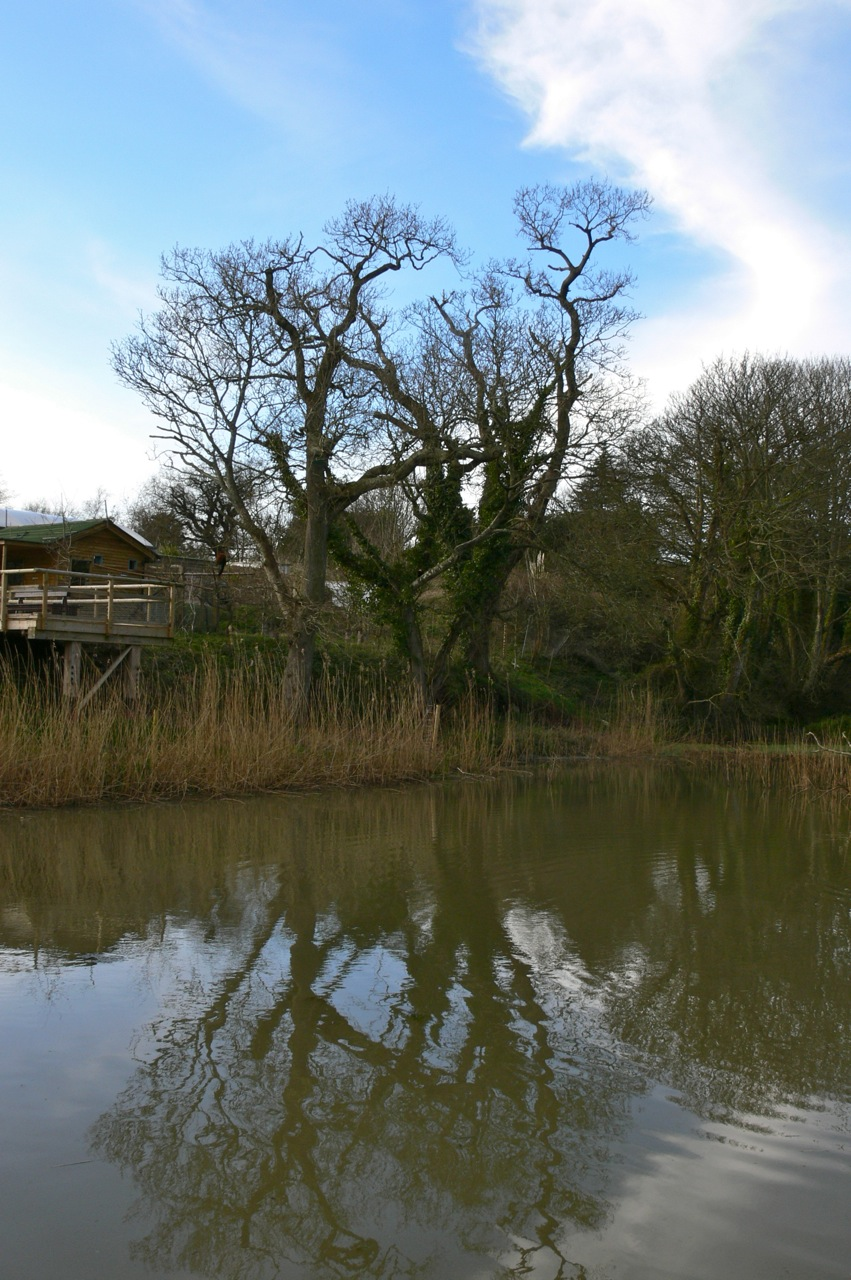
\includegraphics[height=.8\textheight]{img+txt/jersey_zoo_baum.jpg}
          \quad
          \Emph{?}
          \par
        \end{Huge}
      \end{center}

      \note{
        \textbf{8:33}

        \par
      }
    \end{frame}

  % ------------------------------------------------------------------------------------------
    \begin{frame}
      \frametitle{Datenstruktur: Baum}
      
      \hspace*{\fill}
      \Bsp
      \par\bigskip\bigskip
      Repräsentation im Baum ist naheliegend:
      \begin{center}
        \Fig{1}
      \end{center}

      \note{
        \textbf{8:33}

        \par
      }
    \end{frame}

  % ------------------------------------------------------------------------------------------
    \begin{frame}
      \frametitle{Datenstruktur: Baum}
      
      \hspace*{\fill}
      \Bsp
      \par\bigskip\bigskip
      \Emph{Ist das derselbe oder ein anderer Baum?}\Phantom{g}
      \begin{center}
        \Fig{2}
      \end{center}

      \note{
        \textbf{8:34}

        \par
      }
    \end{frame}

  % ------------------------------------------------------------------------------------------
    \begin{frame}
      \frametitle{Automaten auf endlichen Bäumen}
      
      \dots\ sind wichtig für semistrukturierte Daten, weil sie \dots
      \begin{Itemize}
        \item
          XML-Schemasprachen und -validierung zugrunde liegen
        \item
          XML-Anfragesprachen auf ihnen aufgebaut sind
      \end{Itemize}


      \note{
        \textbf{8:35}

        \par
      }
    \end{frame}

  % ------------------------------------------------------------------------------------------
    \begin{frame}
      \frametitle{XML-Schemasprachen und -validierung}
      
      \begin{Itemize}
        \item
          Schemasprachen zur Beschreibung gültiger Bäume
        \item
          Validierung $=$ Erkennen gültiger und ungültiger Bäume
        \item
          gängige Schemasprachen benutzen dafür Baumautomaten
      \end{Itemize}
      
      \par\bigskip
      \uncover<2->{%
        \Gmph{Beispiel:}
%         \begin{Itemize}
%           \setbeamercolor{local structure}{parent=example text}
%           \item
            jeder Name muss einen Vor- und Nachnamen haben
%         \end{Itemize}
        \begin{center}
          \Fig{10}~
          \uncover<3->{{\Huge \YES}}
          \qquad
          \uncover<4->{\Fig{11}}~
          \uncover<5->{{\Huge \NO}}
        \end{center}
      }

      \note{
        \textbf{8:35}

        \par
      }
    \end{frame}

  % ------------------------------------------------------------------------------------------
    \begin{frame}
      \frametitle{XML-Anfragesprachen}
      
      \begin{Itemize}
        \item
          beantworten Anfragen mit Daten aus gegebenen Bäumen
      \end{Itemize}

      \par\bigskip
      \uncover<2->{%
        \Gmph{Beispiel:}
%         \begin{Itemize}
%           \setbeamercolor{local structure}{parent=example text}
%           \item
            gib alle Namen von Personen zurück
%         \end{Itemize}
        \begin{center}
          \Fig{3}
          \quad
          \Fig{12}
        \end{center}
      }

      \note{
        \textbf{8:36}

        \par
      }
    \end{frame}

%   % ------------------------------------------------------------------------------------------
%     \begin{frame}
%       \frametitle{\dots}
%       \dots
%     \end{frame}
% 
%%%  }

  % ==============================================================================================
  % ==============================================================================================
  \section{Grundbegriffe}

%%%  \mysectioncontent{%
  % ------------------------------------------------------------------------------------------
    \begin{frame}
      \frametitle{Positionen im Baum}
      \begin{Itemize}
        \item
          \Emph{positive} natürliche Zahlen: $\mathbb{N}_+$
        \item
          \Bmph{Position:} Wort $p \in \mathbb{N}_+^*$
      \end{Itemize}
      
      \par\bigskip
      \Bmph{Idee:} Wurzel ist $\varepsilon$ \\
      \hspace*{7mm} $j$-ter Nachfolger von $p$ ist $pj$
      
      \par\bigskip
      \Gmph{Beispiel:}
      \begin{center}
        \Fig{20}
      \end{center}

      \note{
        \textbf{8:37}

        \par
      }
    \end{frame}

  % ------------------------------------------------------------------------------------------
    \begin{frame}
      \frametitle{Alphabet mit Stelligkeit}
      
      \begin{Itemize}
        \item
          hier: \Bmph{r-Alphabet} $\Sigma$
          \quad
          (auf Englisch: \emph{ranked alphabet})
        \item
          nichtleere endliche Menge von Symbolen;\\
          jedem Symbol ist eine Stelligkeit $\in \mathbb{N}$ zugeordnet
        \item
          $\Sigma_m = \text{Menge der Symbole mit Stelligkeit $m$}$
        \item
          Schreibweise: $\Sigma = \{a_1/r_1,\dots,a_n/r_n\}$ heißt:\\
          $\Sigma$ enthält die Symbole $a_i$ mit Stelligkeit $r_i$, $i=1,\dots,n$
      \end{Itemize}

      \par\bigskip
      \uncover<2->{%
        \Gmph{Beispiel:} $\Sigma = \{a/2,~ b/3,~ c/0,~ d/0\}$
        \begin{center}
          \begin{minipage}{.2\textwidth}
            \Fig{20}
          \end{minipage}
          \hfill
          \begin{minipage}{.45\textwidth}
            \begin{small}
              $a$ "`passt"' in Position $2$ \\
              $b$ "`passt"' in Position $\varepsilon$ \\
              $c,d$ "`passen"' in Pos.\ $1,21,22,3$
            \par
            \end{small}
          \end{minipage}
          \hfill
          \uncover<3->{%
            $\leadsto$
            \hfill
            \begin{minipage}{.2\textwidth}
              \Fig{21}
            \end{minipage}
            \par
            \begin{small}
              \par\medskip
              \hspace*{\fill}Baum über $\Sigma$ \qquad
            \end{small}%
          }
        \end{center}
      }

      \note{
        \textbf{8:38}

        \par
%        \textbf{Fragebogen F.\ 3a}
        
      }
    \end{frame}

  % ------------------------------------------------------------------------------------------
    \begin{frame}[t]
      \frametitle{Was ist nun ein Baum?}

      \begin{center}
        \begin{Huge}
          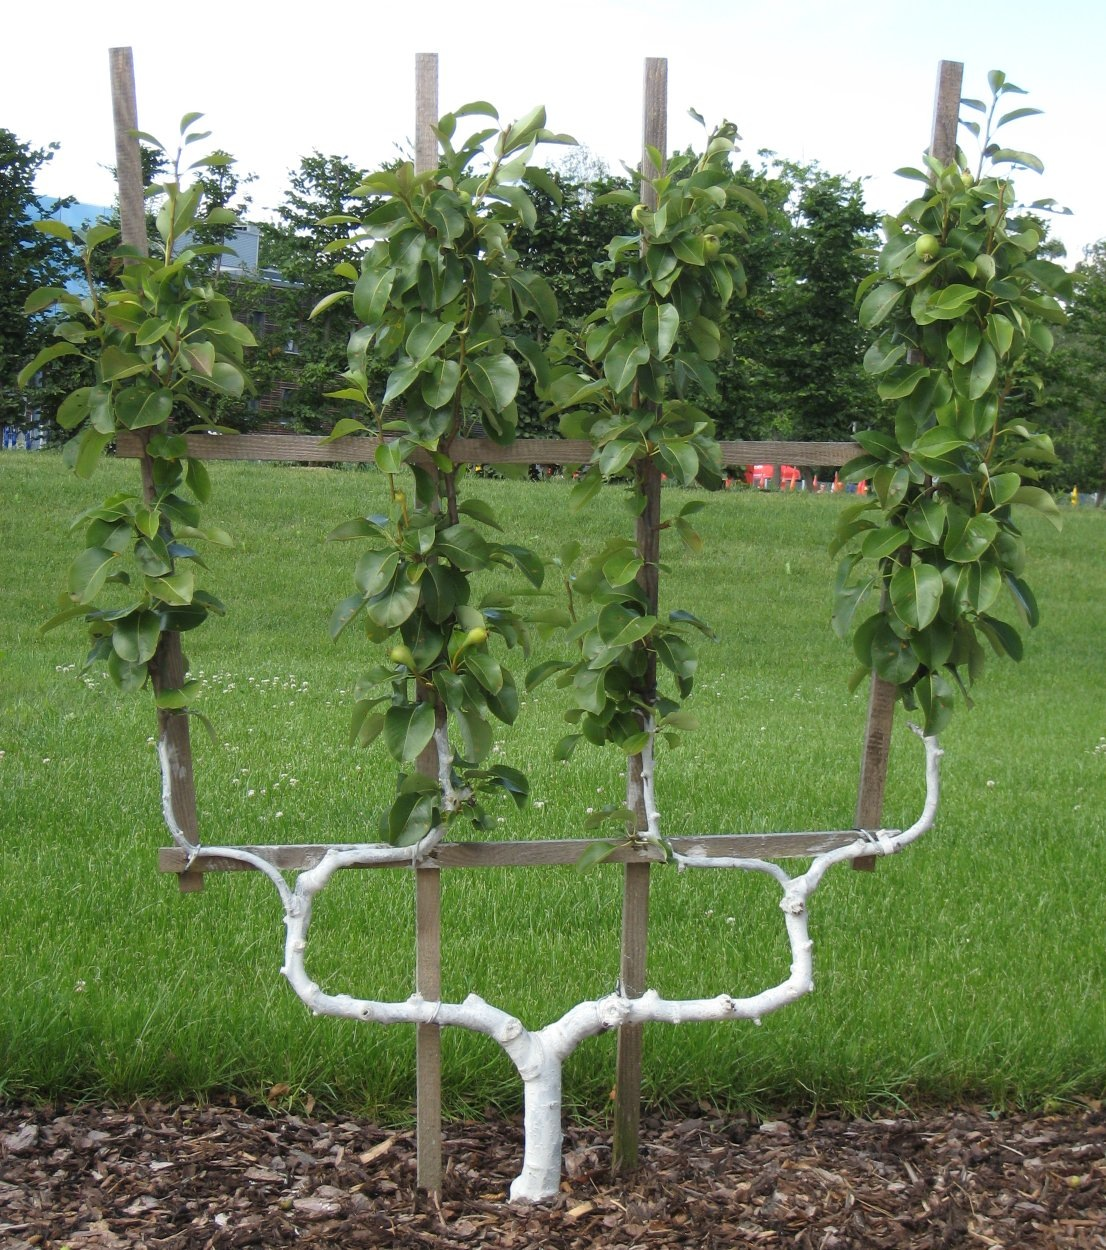
\includegraphics[height=.8\textheight]{img+txt/binary_tree.jpg}
          \quad
          \Emph{?}
          \par
        \end{Huge}
      \end{center}

      \note{
        \textbf{8:42}

        \par
      }
    \end{frame}

  % ------------------------------------------------------------------------------------------
    \begin{frame}%[t]
      \frametitle{Was ist ein Baum?}
      
      \begin{Definition}
        Ein \Bmph{endlicher geordneter Baum} über dem r-Alphabet $\Sigma$ ist ein Paar $T = (P,t)$, wobei
        \begin{Enumerate}
          \item[\Bmph{(1)}]
            $P \subseteq \mathbb{N}_+^*$ eine nichtleere endl.\ präfix-abgeschlossene Menge ist,
          \item[\Bmph{(2)}]
            $t : P \to \Sigma$ eine Funktion ist mit den folgenden Eigenschaften.
            \begin{Enumerate}
              \item[\Bmph{(a)}]
                Wenn $t(p) \in \Sigma_0$, dann $\{j \mid pj \in P\} = \emptyset$.
              \item[\Bmph{(b)}]
                Wenn $t(p) \in \Sigma_m$, $m\geqslant 1$,
                dann $\{j \mid pj \in P\} = \{1,\dots,m\}$.
            \end{Enumerate}
        \end{Enumerate}
      \end{Definition}
      
      \par\medskip
      \uncover<2->{%
        \Bmph{Erklärungen:}
        \begin{Enumerate}
          \item[\Bmph{(1)}]
            $P$: Menge der vorhandenen Positionen
          \item[]
            Präfix-Abgeschlossenheit: Baum ist wohlgeformt\\
            {\small (z.\,B.: wenn Position 31 existiert, dann auch Position 3 und $\varepsilon$)}
          \item[\Bmph{(2)}]
            \Bmph{(a)} und \Bmph{(b)} sagen:~ Stelligkeit des Zeichens an Position $p$
            muss mit der Anzahl der Kinder von $p$ übereinstimmen.
        \end{Enumerate}
      }


      \note{
        \textbf{8:42}

        \par
      }
    \end{frame}

  % ------------------------------------------------------------------------------------------
    \begin{frame}%[t]
      \frametitle{Was ist ein Baum?}
%       \addtocounter{theorem}{-1}
%       \begin{Definition}
%         Ein \Bmph{endlicher geordneter Baum} über dem r-Alphabet $\Sigma$ ist ein Paar $T = (P,t)$, wobei
%         \begin{Itemize}
%           \item
%             $P \subseteq \mathbb{N}_+^*$ eine nichtleere endl.\ präfix-abgeschlossene Menge ist,
%           \item
%             $t : P \to \Sigma$ eine Funktion ist mit den folgenden Eigenschaften.
%             \begin{Enumerate}
%               \item
%                 Wenn $t(p) \in \Sigma_0$, dann $\{j \mid pj \in P\} = \emptyset$.
%               \item
%                 Wenn $t(p) \in \Sigma_m$, $m\geqslant 1$,
%                 dann $\{j \mid pj \in P\} = \{1,\dots,m\}$.
%             \end{Enumerate}
%         \end{Itemize}
%       \end{Definition}
      
      \par\medskip
      \Bmph{Bezeichnungen}
      \begin{Itemize}
        \item
          Position $p$ hat \Bmph{Kinder} $p1,p2,\dots$;\\
          $p$ ist deren \Bmph{Elternteil} 
          \par\smallskip
        \item
          jedes Präfix von $p$ ist ein \Bmph{Vorgänger} von $p$; \\
          $p$ ist \Bmph{Nachfolger} eines jeden Präfixes von $p$
          \par\smallskip
        \item
          \Bmph{Blatt:}~ Knoten ohne Kinder
          \par\smallskip
        \item
          \Bmph{Höhe von $p$} in $T$:\\
          Länge des längsten Pfades von $p$ zu einem Blatt
          \par\smallskip
        \item
          \Bmph{Höhe von $T$}:~ Höhe von $\varepsilon$ in $T$
      \end{Itemize}

      \note{
        \textbf{8:45}

        \par
      }
    \end{frame}

  % ------------------------------------------------------------------------------------------
    \begin{frame}
      \label{frame:baumbeispiel}
      \frametitle{Beispiel}
      ~\par\vspace*{-2\baselineskip}
      \begin{align*}
        \Sigma &= \{a/2,~ b/3,~ c/0,~ d/0\} \\
        P      &= \{\varepsilon, 1,2,3,21,22\} \\[4mm]
        t(\varepsilon) &= b,~ t(1) = c,~ t(2) = a,~ t(3) = c,~ t(21) = c,~ t(22) = d
      \end{align*}

      \par\smallskip
      \begin{center}
        \parbox{.20\textwidth}{%
          \begin{small}
            \strut Positionen $P$
            \par\smallskip
          \end{small}
          \Fig{20}%
        }%
        \quad
        \parbox{.24\textwidth}{%
          \begin{small}
            \strut Baum $T=(P,t)$
            \par\smallskip
          \end{small}
          \Fig{21}%
        }%
        \qquad
        \parbox{.36\textwidth}{%
          \begin{small}
            andere Schreibweise:\\
            \[
              b(ca(cd)c)
            \]
            ($\approx$ in-order-Tiefensuche)
          \end{small}%
        }
      \end{center}

      \begin{Itemize}
        \item
          Höhe: 2
%         \item
%           Wurzelsymbol: $b$
        \item
          Blätter: 1, 21, 22, 3
        \item
          $21$ ist Kind von $2$ und hat Vorgänger $2$, $\varepsilon$
      \end{Itemize}


      \note{
        \textbf{8:46}

        \par
      }
    \end{frame}

  % ------------------------------------------------------------------------------------------
    \begin{frame}
      \frametitle{Bottom-up-Baumautomaten}
      \begin{definition}
        Ein \Bmph{nichtdet.\ Bottom-up-Automat auf endl.\ geord.\ Bäumen (NEBA)}\\
        ist ein Quadrupel $\Aut{A} = (Q,\Sigma,\Delta,F)$, wobei
        \begin{Itemize}
          \item
            $Q$ eine endliche nichtleere \Bmph{Zustandsmenge} ist,
          \item
            $\Sigma$ ein r-Alphabet ist,
          \item
            $\Delta$ eine Menge von \Bmph{Überführungsregeln} der Form
            \[
                a(q_1,\dots,q_m) \to q
            \]
            ist mit $m \geqslant 0$,\quad $a \in \Sigma_m$,\quad $q,q_1,\dots,q_m \in Q$,\quad und
          \item
            $F \subseteq Q$ die Menge der \Bmph{akzeptierenden Zustände} ist.
        \end{Itemize}%
        \label{def:NEBA}%
        \vspace*{-2mm}
      \end{definition}

      \note{
        \textbf{8:50}

        \par\medskip
        Keine Anfangszustände -- wir sehen gleich, warum.
        
        \par
      }

    \end{frame}

  % ------------------------------------------------------------------------------------------
    \begin{frame}
      \frametitle{Bottom-up-Baumautomaten: Intuitionen}
      
%       \Bmph{Zur Erinnerung:}
%       NEBA ist ein Quadrupel $\Aut{A} = (Q,\Sigma,\Delta,F)$ mit
%       \begin{block}{}
%         \begin{Itemize}
%           \item
%             $Q$:\quad endliche nichtleere Zustandsmenge
%           \item
%             $\Sigma$:\quad r-Alphabet
%           \item
%             $\Delta$:\quad Menge von Überführungsregeln
%             \quad
%             $
%                 a(q_1,\dots,q_m) \to q
%             $\\
%             \qquad ($m \geqslant 0$,\quad $a \in \Sigma_m$,\quad $q,q_1,\dots,q_m \in Q$)
%           \item
%             $F \subseteq Q$:\quad Menge der Endzustände
%         \end{Itemize}
%       \end{block}
      
%       \par\bigskip
%       \uncover<2->{%
        \Bmph{Bedeutung der Überführungsregeln $a(q_1,\dots,q_m) \to q$\,:} 
%         \par\smallskip
%         wenn $\Aut{A}$
        \begin{Itemize}
          \item
            Wenn \Aut{A} in Position $p$ Zeichen $a$ liest
          \item
            und in $p$'s Kindern Zustände $q_1,\dots,q_m$ eingenommen hat,
        \end{Itemize}
        dann darf $\Aut{A}$ in $p$ Zustand $q$ einnehmen.
%        \hfill{\small (Skizze siehe Tafel)} 
        \Tafel

%       }
%     \end{frame}
% 
%   % ------------------------------------------------------------------------------------------
%     \begin{frame}[t]
%       \frametitle{Bottom-up-Baumautomaten: Intuitionen}
%       
%       \Bmph{Zur Erinnerung:}
%       NEBA ist ein Quadrupel $\Aut{A} = (Q,\Sigma,\Delta,F)$ mit
%       \begin{block}{}
%         \begin{Itemize}
%           \item
%             $Q$:\quad endliche nichtleere Zustandsmenge
%           \item
%             $\Sigma$:\quad r-Alphabet
%           \item
%             $\Delta$:\quad Menge von Überführungsregeln
%             \quad
%             $
%                 a(q_1,\dots,q_m) \to q
%             $\\
%             \qquad ($m \geqslant 0$,\quad $a \in \Sigma_m$,\quad $q,q_1,\dots,q_m \in Q$)
%           \item
%             $F \subseteq Q$:\quad Menge der Endzustände
%         \end{Itemize}
%       \end{block}
      
      \par\bigskip\smallskip
      \uncover<2->{%
        \Bmph{$\leadsto$ Andere Betrachtungsweise:}
        \begin{Itemize}
          \item
            $\Aut{A}$ markiert Eingabebaum $T$ \Emph{bottom-up} mit Zuständen
          \item
            $\Aut{A}$ akzeptiert $T$, wenn $\Aut{A}$ in der Wurzel einen akzeptierenden Zustand einnimmt
        \end{Itemize}
      }
% 
%     \end{frame}
% 
%     % ------------------------------------------------------------------------------------------
%     \begin{frame}[t]
%       \frametitle{Bottom-up-Baumautomaten: Intuitionen}
%       
%       \Bmph{Zur Erinnerung:}
%       NEBA ist ein Quadrupel $\Aut{A} = (Q,\Sigma,\Delta,F)$ mit
%       \begin{block}{}
%         \begin{Itemize}
%           \item
%             $Q$:\quad endliche nichtleere Zustandsmenge
%           \item
%             $\Sigma$:\quad r-Alphabet
%           \item
%             $\Delta$:\quad Menge von Überführungsregeln
%             \quad
%             $
%                 a(q_1,\dots,q_m) \to q
%             $\\
%             \qquad ($m \geqslant 0$,\quad $a \in \Sigma_m$,\quad $q,q_1,\dots,q_m \in Q$)
%           \item
%             $F \subseteq Q$:\quad Menge der Endzustände
%         \end{Itemize}
%       \end{block}
      
      \par\bigskip
      \uncover<3->{%
        \Bmph{Was sind dann die Anfangszustände?}
        \begin{Itemize}
          \item<4->
            Ü-Regeln $a() \to q$ deklarieren "`zeichenspezifische"' AZ:\\
            $\Aut{A}$ darf in mit $a$ markierten Blättern in $q$ starten
          \item<4->
            Kurzschreibweise: $a \to q$
        \end{Itemize}
      }
    
      \note{
        \textbf{8:52 bis 8:56}

        \par\medskip
        \textbf{Fragen:}~ Was sind dann die Anfangszustände?
                
%        \par\medskip
%        \textbf{Fragebogen F.\,3b$+$c}
        
        \par
      }
    \end{frame}

    % ------------------------------------------------------------------------------------------
    \begin{frame}[t]
      \frametitle{Berechnungen \qquad {\normalsize (analog zu NEAs)}}
      \begin{Definition}
        Sei $\Aut{A} = (Q,\Sigma,\Delta,F)$ ein NEBA und $T=(P,t)$ ein $\Sigma$-Baum.
        \begin{Itemize}
          \item
            Ein \Bmph{Run} von \Aut{A} auf $T$
            ist eine Fkt.\ $r : P \to Q$ mit:
            \begin{Itemize}
              \item
                Wenn $t(p) = a \in \Sigma_0$ und $r(p) = q$, dann $a \to q \in \Delta$.
              \item<2->
                Wenn $t(p) = b \in \Sigma_m$ $(m \geqslant 1)$ und $r(p) = q$ \\
                und wenn $r(p1) = q_1$,\quad \dots,\quad $r(pm) = q_m$,
                \par\smallskip
                \uncover<3->{%
                  dann $b(q_1,\dots,q_m) \to q \in \Delta$.%
                }
            \end{Itemize}
        \end{Itemize}
        \label{def:berechnung_NEBA}%
        \vspace*{-2mm}
      \end{Definition}
      
      \par\bigskip
      \uncover<4->{%
        \Bmph{Also gilt:}
        \begin{Itemize}
          \item
            Blatt mit $a$ kann $q$ nur zugewiesen kriegen, wenn $a \to q \in \Delta$.
          \item<5->
            Nicht-Blatt mit $b$, dessen Kinder $q_1,\dots,q_m$ haben,\\
            kann $q$ nur zugew.\ kriegen, wenn $b(q_1,\dots,q_m) \to q \in \Delta$.
        \end{Itemize}
      }

      \note{
        \uz{8:56 $\to$ 5\,min Puffer $\to$ 9:01}
        
        \par
      }
    \end{frame}

    % ------------------------------------------------------------------------------------------
    \begin{frame}[t]
      \frametitle{Berechnungen, Akzeptanz und erkannte Sprache}
      \begin{block}{Definition \ref{def:berechnung_NEBA}}
        Sei $\Aut{A} = (Q,\Sigma,\Delta,F)$ ein NEBA und $T=(P,t)$ ein $\Sigma$-Baum.
        \begin{Itemize}
          \item
            Ein \Bmph{Run} von \Aut{A} auf $T$
            ist eine Funktion $r : P \to Q$ mit:
            \begin{Itemize}
              \item
                Wenn $t(p) = a \in \Sigma_0$ und $r(p) = q$, dann $a \to q \in \Delta$.
              \item
                Wenn $t(p) = b \in \Sigma_m$ $(m \geqslant 1)$ und $r(p) = q$ \\
                und wenn $r(p1) = q_1$,\quad \dots,\quad $r(pm) = q_m$,
                \par\smallskip
                dann $b(q_1,\dots,q_m) \to q \in \Delta$.%
            \end{Itemize}
            \par\smallskip
          \item
            Ein Run $r$ von \Aut{A} auf $T$ ist \Bmph{erfolgreich}, wenn $r(\varepsilon) \in F$.
          \item
            \Aut{A} \Bmph{akzeptiert} $T$, wenn es einen erfolgreichen Run von \Aut{A} auf $T$ \Emph{gibt}.
          \item
            Die von \Aut{A} \Bmph{erkannte Sprache} ist
            \par
            $L(\Aut{A}) = \{T \text{~über~} \Sigma \mid \Aut{A} \text{~akzeptiert~} T\}$.
        \end{Itemize}
      \end{block}

      \note{%
        \uz{9:04}
        
        \par
      }
    \end{frame}

    % ------------------------------------------------------------------------------------------
    \begin{frame}
      \frametitle{Beispiel 1}

      \begin{Itemize}
        \item
          Sei $\Sigma = \{a/2, b/0, c/0\}$ und $\Aut{A} = (\{q_0,\dots,q_3\}, \Sigma, \Delta, \{q_2\})$
          \begin{align*}
            \text{mit}~ \Delta & = \{~b \to q_0,\quad c \to q_0, \\
                               & \qquad ~a(q_0,q_0) \to q_1,      \\
                               & \qquad ~a(q_1,q_1) \to q_2,\quad a(q_1,q_1) \to q_3~\}.
          \end{align*}
          \par\smallskip
        \item<2->
          Dann gibt es auf dem Baum
          \begin{center}
            \begin{minipage}{.21\textwidth}
              \Fig{31}
            \end{minipage}
            \quad
            2 Runs:
            \quad
            \uncover<3,5->{%
              \begin{minipage}{.21\textwidth}
                \Fig{32}
              \end{minipage}%
            }
            \uncover<4->{%
              \quad
              \begin{minipage}{.21\textwidth}
                \Fig{33}
              \end{minipage}%
            }
          \end{center}
          \par\bigskip
        \item<6->
          $L(\Aut{A}) =$
          \only<6|handout:0>{?}%
          \only<7->{$\{T \text{~über~} \Sigma \mid \text{alle Pfade in $T$ haben Länge 2}\}$}
          \par\bigskip
        \item<8->
          \Bmph{Anmerkung:} Da $\Sigma$ nur $./2$ und $./0$ enthält:
          \par\smallskip
          \scalebox{.95}[1]{%
            $L(\Aut{A}) = \{T \text{~über~} \Sigma \mid T \text{~ist der vollständige Binärbaum der Tiefe 2}\}$%
          }
%          \vspace*{-18.26pt}
      \end{Itemize}

      \note{%
        \uz{9:05}
        
        \parII
        \textbf{Fragen:}~ Welche Runs gibt es?\quad Was ist die erkannte Sprache?
        
        \par
      }
    \end{frame}

    % ------------------------------------------------------------------------------------------
    \begin{frame}
      \frametitle{Beispiel 2}

      Sei $\Sigma = \{a/2,~ b/1,~ c/0,~ d/0\}$.\quad Welcher NEBA erkennt
      \par\smallskip
      $\{T \text{~über~} \Sigma \mid \text{~jedes $c$-Blatt hat ein rechtes $d$-Geschwister}\}$?

      \par\bigskip
      \uncover<2->{%
        $\Aut{A} = (\{q_c,q_d,q_f\},\Sigma,\Delta,\{q_f\})$ mit
%         \begin{alignat*}{3}
%           \Delta & = \{   ~& c          & \to q_0, &      b(q_0)     & \to m,  \\
%                  & \qquad ~& d          & \to q_1, &\quad a(q_0,q_0) & \to m,  \\
%                  & \qquad ~& a(q_0,q_1) & \to q_1, &      b(m)       & \to m,  \\
%                  & \qquad ~& a(q_1,q_0) & \to q_1, &      a(m,m)     & \to m,  \\
%                  & \qquad ~& b(q_1)     & \to q_1, &      a(q_0,m)   & \to m,  \\
%                  & \qquad ~& a(q_1,q_1) & \to q_1, &      a(m,q_0)   & \to m,  \\
%                  &         &            &          &      a(q_1,m)   & \to m,  \\
%                  &         &            &          &      a(m,q_1)   & \to m~\}
%         \end{alignat*}
%        \begin{alignat*}{3}
%          \Delta & = \{   ~& c          & \to q_c,  & \quad a(q_c,q_d) & \to q_f,  \\
%                 & \qquad ~& d          & \to q_d,  &      & \\ % a(q_d,q_d) & \to q_f,  \\
%                 & \qquad ~& d          & \to q_f,  &      & \\[4pt] % a(q_d,q_f) & \to q_f,  \\
%%                  &         &            &           &      a(q_f,q_d) & \to q_f,  \\[4pt]
%                 & \qquad ~& b(q_f)     & \to q_f,  &      a(q_f,q_f) & \to q_f~\}
%        \end{alignat*}
        \begin{alignat*}{4}
          \Delta & = \{   ~& c          & \to q_c,  & \quad d    & \to q_d, & \quad d          & \to q_f, \\
                 & \qquad ~& a(q_c,q_d) & \to q_f,  &            &          &                  &          \\
                 & \qquad ~& a(q_f,q_f) & \to q_f,  &            &          &                  &          \\
                 & \qquad ~& b(q_f)     & \to q_f   & ~\}        &          &                  & 
        \end{alignat*}
      }
        
      \par\smallskip
      \uncover<3->{%
        \begin{small}
          Übergang $a(q_d,q_d) \to q_f$ ist überflüssig: $d \to q_f$ und $a(q_f,q_f) \to q_f$.
          \par
        \end{small}
      }
      
      \par\bigskip
      \uncover<4->{%
        Beispielbaum und -run:~ siehe Tafel \Tafel
      }

      \note{%
        \uz{9:08 bis 9:15}
        
        \parII
        Gemeinsam machen, Zeit nehmen!
        
        \par
      }
    \end{frame}

    % ------------------------------------------------------------------------------------------
    \begin{frame}
      \frametitle{Erkennbare Baumsprache}
      
      \begin{Definition}
        Eine Menge $L$ von (endlichen geordneten) Bäumen über $\Sigma$
        \par
        ist eine \Bmph{erkennbare Baumsprache},
        \par\smallskip
        wenn es einen NEBA \Aut{A} gibt mit $L(\Aut{A}) = L$.
      \end{Definition}


      \note{%
        \uz{9:15, 5\,min Pause bis 9:20}
        
        \par
      }
    \end{frame}

    % ------------------------------------------------------------------------------------------
    \begin{frame}
      \frametitle{Determinismus}

      \begin{Definition}
        Sei $\Aut{A} = (Q,\Sigma,\Delta,F)$ ein NEBA.
        \par\smallskip
        Enthält $\Delta$ für jedes jedes $a \in \Sigma_m$ und alle $(q_1,\dots,q_m) \in Q^m$
        \par
        \Emph{höchstens eine}\footnote[frame]{hier "`höchstens eine"' statt "`genau eine"': vermeidet Papierkorbzustand}
        Regel $a(q_1,\dots,q_m) \to q$
        \par\smallskip
        dann ist \Aut{A} ein \Bmph{deterministischer endlicher Baumautomat (DEBA)}.
      \end{Definition}

      \begin{Itemize}
        \item<2->[$\leadsto$]
          Nachfolgezustand für jedes $(m+1)$-Tupel $a(q_1,\dots,q_m)$ \\
          ist eindeutig bestimmt (wenn er existiert)
        \item<2->
          Jeder DEBA ist ein NEBA,\\
          aber nicht umgekehrt %\\
%           \hspace*{38.5mm}
          {\small (z.\,B.\ die vergangenen 2 Beispiele)}.
      \end{Itemize}

      \uncover<3->{%
        \begin{alertblock}{Frage}
          Sind DEBAs und NEBAs gleichmächtig?
        \end{alertblock}
      }
    
      \note{%
        \uz{9:20}
        
        \parII
        Determinismus, "`höchstens eine Regel \dots"':~ \\
        Papierkorbzustand $q^-$ ist hier umständlicher als bei NEAs: \\
        $\bullet$ mehr Kombis $a(q_1,\dots,q_m) \to q^-$ \\
        $\bullet$ man brauchte bei $m$-stelligen Zeichen $a$ lange Regel $a(q^-,\dots,q^-) \to q^-$
        
        \par\bigskip
        Beispiele:~ \textbf{beide} Aut.\ sind NEBAs.
        
        \par\bigskip
        \textbf{Frage} stellen!
        
        \par
      }
    \end{frame}

    % ------------------------------------------------------------------------------------------
    \begin{frame}
      \frametitle{Potenzmengenkonstruktion}

      \Gmph{Antwort:~} Ja!

      \par\smallskip
      \begin{Satz}
        Für jeden NEBA $\Aut{A}$ gibt es einen DEBA $\Aut{A}^d$ mit $L(\Aut{A}^d) = L(\Aut{A})$.
        \label{thm:potenzmengenkonstruktion}%
      \end{Satz}

      \par\smallskip
      \uncover<2->{%
        \Bmph{Beweis:}\qquad {\small (analog zur Potenzmengenkonstr.\ für NEAs)}
        
        Sei $\Aut{A} = (Q,\Sigma,\Delta,F)$.~
%        \par\smallskip
        Konstruieren $\Aut{A}^d = (Q^d,\Sigma,\Delta^d,F^d)$:
        
        \begin{Itemize}
          \item
            $Q^d = 2^Q$\qquad (Potenzmenge der Zustandsmenge)
          \item
            $F^d = \{S \subseteq Q \mid S \cap F \neq \emptyset\}$
          \item
            $a(S_1,\dots,S_m) \to S \in \Delta^d$ \quad \Emph{gdw.} \\
            $S = \{q \mid \exists q_1 \!\!\:\in\!\!\: S_1, \dots, \exists q_m \!\!\:\in\!\!\: S_m : a(q_1,\dots,q_m) \!\!\:\to\!\!\: q \in \Delta\}$
        \end{Itemize}
      }
   
      \par\smallskip
      \uncover<3->{%
        $\Aut{A}^d$ ist DEBA (klar) mit $L(\Aut{A}^d) = L(\Aut{A})$.
        \hfill \Tafel
        \qed
      }

      \par\bigskip
      \uncover<3->{%
        Auch für NEBAs kann die Potenzmengenkonstruktion \\
        im schlimmsten Fall zu exponentiell vielen Zuständen führen.%
      }


      \note{%
        \uz{9:23 bis 9:50? $\to$ 10\,min Reserve}
        
        \parII
        ``ist DEBA'':~ sogar genau 1 Folgezustand statt ``höchstens 1''
        
        \par
      }
    \end{frame}

%   % ==============================================================================================
%   % ==============================================================================================
%   \section[Determinis.]{Determinisierung}
% 
%   % ------------------------------------------------------------------------------------------
%     \begin{frame}
%       \frametitle{\dots}
%       \dots
%     \end{frame}

%%%  }
  
%   % ==============================================================================================
%   % ==============================================================================================
%   \section[\protect\emph{Anw.\ 1}]{\protect\emph{Anwendung 1: Einschließung bei Termersetzungssystemen}}
% 
%%%%   \mysectioncontent{%
%     % ------------------------------------------------------------------------------------------
%     \begin{frame}
%       \frametitle{Motivation: Termersetzungssysteme \dots}
% 
%       \begin{Itemize}
%         \item
%           sind ein mächtiges Berechnungsmodell (Turing-vollständig)
%         \item
%           liegen u.\,a.\ Logik- und funktionaler Programmierung zugrunde
% %         \item<2->
% %           bestehen aus Regeln zur Ersetzung von Termen:
%       \end{Itemize}
%       
%       \begin{Beispiel}<2->[symbolische Addition natürlicher Zahlen]
%         \begin{Itemize}
%           \item
%             $0,1,2,\dots$ werden dargestellt als $0,\Succ(0),\Succ(\Succ(0)),\dots$
%           \item<3->
%             Ersetzungsregeln:
%             \begin{center}
%               \begin{small}
%                 \begin{tabular}{@{~~}lrcl@{~~}}
%                   R1 & $\Plus(0,y)$        & $\to$ & $y$                 \\
%                   R2 & $\Plus(\Succ(x),y)$ & $\to$ & $\Succ(\Plus(x,y))$
%                 \end{tabular}
%                 \par
%               \end{small}
%             \end{center}
%           \item<4->
%             Anwendung auf Beispielausdruck:
%             \par\vspace*{-1.4\baselineskip}
%             \begin{small}
%               \begin{align*}
%                 \Plus(\Succ(\Plus(0,\Succ(0))),\Succ(0))
%                 & \stackrel{\rule[-2pt]{0pt}{1pt}\text{R1}}{\mapsto} \Plus(\Succ(\Succ(0)),\Succ(0)) \\
%                 & \stackrel{\rule[-2pt]{0pt}{1pt}\text{R2}}{\mapsto} \Succ(\Plus(\Succ(0),\Succ(0))) \\
%                 & \stackrel{\rule[-2pt]{0pt}{1pt}\text{R2}}{\mapsto} \Succ(\Succ(\Plus(0,\Succ(0)))) \\
%                 & \stackrel{\rule[-2pt]{0pt}{1pt}\text{R1}}{\mapsto} \Succ(\Succ(\Succ(0)))
%               \end{align*}
%               \par
%             \end{small}
%         \end{Itemize}
% 
%       \end{Beispiel}
% 
% 
%     \end{frame}
% 
%   % ------------------------------------------------------------------------------------------
%     \begin{frame}
%       \label{frame:Terme}%
%       \frametitle{Grundbegriffe}
% 
%       \begin{Itemize}
%         \item
%           \Bmph{r-Alphabet} $\Sigma$ wie bekannt (Symbole mit Stelligkeiten)
%         \item
%           endliche Menge $V$ von \Bmph{Variablen} (0-stellig)
%         \item
%           \Bmph{Terme} über $\Sigma,V$, geschrieben $\calT(\Sigma, V)$:
%           \begin{Itemize}
%             \item
%               Alle 0-stelligen Symbole sind Terme:~ $\Sigma_0 \cup V \subseteq \calT(\Sigma, V)$
%             \item
%               Wenn $m \geqslant 1$, $a \in \Sigma_m$ und $t_1, \dots, t_m \in \calT(\Sigma, V)$,
%               \par
%               dann $a(t_1,\dots,t_m) \in \calT(\Sigma, V)$.
%           \end{Itemize}
%         \item
%           \Bmph{Grundterme:} variablenfreie Terme
%       \end{Itemize}
%       
%       \par\bigskip
%       \uncover<2->{%
%         \Gmph{Beobachtung:}
%         Terme sind nur eine andere Schreibweise für Bäume.
%         \begin{center}
%           \begin{minipage}{.70\textwidth}
%             \begin{small}
%               $\Plus(\Succ(\Plus(0,\Succ(0))),\Succ(0))$
%               \qquad
%               entspricht
%               \par
%             \end{small}
%           \end{minipage}
%           \qquad
%           \begin{minipage}{.21\textwidth}
%             \Fig{22}
%           \end{minipage}
%         \end{center}
%       }
% 
%     \end{frame}
% 
%   % ------------------------------------------------------------------------------------------
%     \newlength{\bsp}
%     \settowidth{\bsp}{{\small Bsp.:}}
%     \begin{frame}
%       \frametitle{Regeln und deren Anwendung}
% 
%       \Bmph{Termersetzungsregeln} sind Paare $\ell \to r$ mit
%       \begin{Itemize}
%         \item[]
%           $\ell,r \in \calT(\Sigma, V)$ \hfill
%           {\small ($+$ gewisse Einschränkungen, wg.\ Terminierung)}
%       \end{Itemize}
%       
%       \par\bigskip
%       \uncover<2->{%
%         \Bmph{Regelanwendung:}
%         \begin{Itemize}
%           \item
%             \Bmph{Substitution:} partielle Abbildung $\sigma : V \to \calT(\Sigma, V)$
%             \par\vspace*{-2mm}
%             \begin{minipage}{\linewidth}
%               \begin{exampleblock}{}
%                 {\small Bsp.: wenn $t = \Plus(0,y)$ und $\sigma = \{y \mapsto \Succ(0)\}$,}
%                 \par
%                 {\small \hspace{\bsp} dann $t\sigma = \Plus(0,\Succ(0))$}
%               \end{exampleblock}
%             \end{minipage}
%             \par\medskip
%           \item<3->
%             Term $t$ \Bmph{passt in} Term $s$, wenn es Subst.\ $\sigma$ gibt mit $t\sigma = s$.
%             \par\vspace*{-2mm}
%             \begin{minipage}{\linewidth}
%               \begin{exampleblock}{}
% %                 {\small Bsp.: $b(x)$ passt in $b(s(y))$\hfill wegen $\sigma_1 = \{x \mapsto s(y)\}$}
% %                 \par
%                 {\small Bsp.: $\Plus(0,y)$ passt in $\Plus(0,\Succ(0))$\hfill mit $\sigma = \{y \mapsto \Succ(0)\}$}
%               \end{exampleblock}
%             \end{minipage}
%             \par\medskip
%           \item<4->
%             \mbox{$\ell\!\to\!r$ auf $t$ \Bmph{anwendbar}, wenn $\ell$ in einen Subterm $t'$ von $t$ passt.\hspace*{-10mm}}
%             \par
%             \Bmph{Ergebnis:} $t$, wobei $t'$ durch $r\sigma$ ersetzt wurde
%             \par\vspace*{-2mm}
%             \begin{minipage}{\linewidth}
%               \begin{exampleblock}{}
%                 {\small Bsp.: Anwendung von ~$\Plus(0,y) \to y$~ auf ~$\Succ(\uwave{\Plus(0,\Succ(0))})$} \\[-1mm]
%                 {\small \hspace*{54mm} ergibt ~$\Succ(\uwave{\Succ(0)})$~}
%                 \vspace*{-2mm}
%               \end{exampleblock}
%             \end{minipage}
%         \end{Itemize}
%       }
% 
%     \end{frame}
% 
%     % ------------------------------------------------------------------------------------------
%     \begin{frame}
%       \frametitle{Regelanwendbarkeit mittels Baumautomaten entscheiden}
% 
%       Zentrales Entscheidungsproblem für TE-Systeme:
%       
%       \begin{block}{Einschließungsproblem (Encompassment)}
%         Gegeben Grundterm $t$ und Regel $\ell \to r$,
%         \par
%         gibt es einen Subterm $t'$ von $t$, in den $\ell$ passt?
%         \hfill
%         ($t$ \Bmph{schließt} $\ell$ \Bmph{ein}.)
%       \end{block}
%       
%       \par\smallskip
%       Genauer: gibt es Subterm $t'$ von $t$ und Substitution $\sigma$
%       mit $\ell\sigma = t'$?
%       
%       \par\bigskip
%       \uncover<2->{%
%         \begin{Satz}
%           Wenn in $\ell$ jede Variable höchstens einmal vorkommt,
%           \par
%           dann ist $L = \{t \mid t \text{~schließt $\ell$ ein}\}$ NEBA-erkennbar.
%           \par\medskip
%           $L$ wird sogar durch einen NEBA mit $O(|\ell|)$ Zuständen erkannt.
%         \end{Satz}
% 
%         \par\bigskip
%         Beweis: siehe Tafel. \Tafel
%       }
% 
%       \par\bigskip
%       \uncover<3->{%
%         Lineare Determinisierung ähnlich wie im 1.\ Teil, Textsuche.
%       }
%     \end{frame}
% 
% %     % ------------------------------------------------------------------------------------------
% %     \begin{frame}
% %       \frametitle{\dots}
% % 
% %       \dots
% %     \end{frame}
% % 
%%%%   }
  
  % ==============================================================================================
  % ==============================================================================================
  \section[Charakt.]{Charakterisierungen erkennbarer Baumsprachen}

%%%  \mysectioncontent{%
    % ------------------------------------------------------------------------------------------
    \begin{frame}
      \frametitle{Nichterkennbare Baumsprachen: Intuitionen}
      
      \Gmph{Beispiel:}
      \begin{Itemize}
        \item
          r-Alphabet $\Sigma = \{a/2,~ b/1,~ c/0\}$
        \item
          Baumautomat $\Aut{A} = (\{q_0,q_1\},\Sigma,\Delta,\{q_0\})$ mit
          \begin{alignat*}{4}
            \Delta & = \{   ~& c & \to q_0, & \quad b(q_0) & \to q_1, & \quad a(q_0,q_0) & \to q_1,    \\
                   & \qquad ~&   &          & \quad b(q_1) & \to q_0, & \quad a(q_1,q_1) & \to q_0~\}.
          \end{alignat*}
        \item[$\leadsto$]
          \begin{tabular}[t]{@{}l@{~}c@{~}l@{}}
            $L(\Aut{A})$ & \uncover<1->{$=$}    & \uncover<2->{\mbox{$\{T \mid \text{alle Wurzel-Blatt-Pfade in $T$ haben gerade Länge}\}$.\hspace*{-7mm}}} \\[1mm]
                         & \uncover<3->{$\neq$} & \uncover<3->{$\{T \mid \text{$T$ hat gerade Höhe}\}$  \Tafel}
          \end{tabular}
      \end{Itemize}

      \par\bigskip
      \uncover<4->{%
%        \begin{alertblock}{Frage: Sind die folgenden Baumsprachen erkennbar?}
        \begin{alertblock}{}
          \Gmph{Frage:} Sind die folgenden Baumsprachen (über $\Sigma$) erkennbar?
%           \setlength{\abovedisplayskip}{0pt}
%           \setlength{\belowdisplayskip}{0pt}
%           \setlength{\abovedisplayshortskip}{0pt}
%           \setlength{\belowdisplayshortskip}{0pt}
          \begin{align*}
                        L_1 & = \{T \mid \text{$T$ hat gerade Höhe}\} \\
            \quad\qquad L_2 & = \{T \mid \text{$T$ ist vollständiger Binärbaum}\} \qquad~~\text{\TafelForts}
          \end{align*}
%             $L_1 = \{T \mid \text{$T$ hat gerade Höhe}\}$ \\ % ~über~ $\Sigma = \{a/2,~ b/1,~ c/0\}$ \\
%             $L_2 = \{T \mid \text{$T$ ist vollständiger Binärbaum}\}$ % ~über~ $\Sigma = \{a/2,~b/0\}$
        \end{alertblock}
%        \TafelForts
%         \par\smallskip
%         \begin{small}
%           \begin{tabular}{@{}l@{~}l@{}}
%             (vollst.\ Binärbaum: & jede nicht-Blattposition $p$ hat genau 2 Kinder $p1,p2$; \\
%                                  & Teilbäume $T_{p1},T_{p2}$ haben dieselbe Höhe)
%           \end{tabular}
%           \par
%         \end{small}
      }
%     \end{frame}
% 
%   % ------------------------------------------------------------------------------------------
%     \begin{frame}
%       \frametitle{Nichterkennbare Baumsprachen: Intuitionen}
%       
%       \begin{alertblock}{Frage: Sind die folgenden Baumsprachen erkennbar?}
%         \setlength{\abovedisplayskip}{0pt}
%         \setlength{\belowdisplayskip}{0pt}
%         \setlength{\abovedisplayshortskip}{0pt}
%         \setlength{\belowdisplayshortskip}{0pt}
%         \begin{align*}
%           L_1 & = \{T \mid \text{$T$ hat gerade Höhe}\} \\
%           L_2 & = \{T \mid \text{$T$ ist vollständiger Binärbaum und hat gerade Höhe}\}
%         \end{align*}
%       \end{alertblock}
%       
      \par\medskip
      \uncover<5->{%
        Antwort: \Gmph{Nein.} \TafelForts
      }

      \note{~}
    \end{frame}
    
  % ------------------------------------------------------------------------------------------
    \begin{frame}
      \frametitle{Pumping-Lemma: Hilfsbegriffe}
      
      \Bmph{Einsetzen von Bäumen ineinander:}
        
      \par\medskip
      \begin{Itemize}
        \item
          \Bmph{Variable}: zusätzliches nullstelliges Symbol $x \notin \Sigma_0$
          \par\smallskip
        \item
          \Bmph{(unärer) Kontext}:
          \par
          Baum über $\Sigma \cup \{x\}$, in dem ein Blatt mit $x$ markiert ist \Tafel
          \par\smallskip
        \item
          \Bmph{trivialer Kontext $C_0$}: Kontext der Höhe $0$\quad ($\Rightarrow$ nur Wurzel)
          \par\smallskip
        \item<2->
          \Bmph{Einsetzen} von Bäumen/Kontexten in Kontexte:
          \begin{Itemize}
            \item
              $C[T]$ $=$ der Baum/Kontext, den man aus $C$ erhält,\\
              indem man die Position von $x$ mit Baum/Kontext $T$ ersetzt \TafelForts
            \item
              $C^n$ induktiv definiert:
              \begin{align*}
                C^0     & = C_0 \\
                C^{n+1} & = C^n[C]
              \end{align*}
          \end{Itemize}
      \end{Itemize}


      \note{
        Wir müssen Bäume ineinander ``stecken'' können. \\
        Dafür brauchen wir eine Markierung für die ``Andockstelle'' (Variable) \\
        und den Begriff des Kontexts (Baum mit Andockstelle).
      }
    \end{frame}

  % ------------------------------------------------------------------------------------------
    \begin{frame}
      \frametitle{Pumping-Lemma}

      \begin{Satz}[Pumping-Lemma]
        Sei $L$ eine NEBA-erkennbare Baumsprache über dem r-Alphabet $\Sigma$.
        \par\medskip
        Dann gibt es eine Konstante $k \in \mathbb{N}$,
        \par
        so dass für alle Bäume $T \in L$ mit $\textup{Höhe}(\!\!\:T) \geqslant k$ gilt:
        \par\smallskip
        \mbox{Es gibt Kontexte $C,D$ mit $D\!\!\:\neq\!\!\:C_0$ und Baum $V$ mit $T\!\!\:=\!\!\:C[D[V]]$,\hspace*{-10mm}}
        \par
        so dass $C[D^i[V]] \in L$ für alle $i \in \mathbb{N}$.
        \label{thm:pumping_lemma}%
      \end{Satz}
%      \Tafel

%      \par\bigskip
%      \uncover<2->{%
%        \Bmph{Beweis:} siehe Tafel. \Tafel \par~\qed%
%      }

      \note{
        \textbf{8:30}
      }
    \end{frame}

    % ------------------------------------------------------------------------------------------
    \begin{frame}
      \frametitle{Beweis des Pumping-Lemmas}
      
      \Bmph{Beweis.}~
      Sei $L$ eine erkennbare Baumsprache, \\
      und sei $\Amc = (Q,\Sigma,\Delta,F)$ ein NEBA mit $L(\Amc) = L$.
      
      \par\bigskip
      \uncover<2->{%
        Wir wählen $k = |Q|$.
      }
      
      \par\bigskip
      \uncover<3->{%
        Sei $T = (P,t) \in L$ ein Baum mit Höhe $\geq k$, \\
        und sei $r$ ein erfolgreicher Run von $\Amc$ auf $T$.
      }

      \par\bigskip
      \uncover<4->{%
        Wegen Höhe $\geq k$ gibt es in $T$ einen Pfad mit $\geq k+1$ Knoten. \\
        Darauf gibt es also zwei Positionen $p_1 \neq p_2$ mit demselben Zustand, \\
        d.\,h.\ $r(p_1)=r(p_2)=q$ für ein $q \in Q$.
      }
      
      \par\bigskip
      \uncover<5->{%
        O.\,B.\,d.\,A.\ ist $p_2 = p_1p_3$ für ein $p_3 \neq \varepsilon$. \Tafel
      }

      \note{
        \textbf{8:32}
      }
    \end{frame}
      
    % ------------------------------------------------------------------------------------------
    \begin{frame}
      \frametitle{Beweis des Pumping-Lemmas}
      
      Seien nun:
      %
      \begin{align*}
        U & ~=~ T_{p_1} \\[4pt]
        C & ~=~ \text{derjenige Kontext mit~} C[U] = T \\[4pt]
        V & ~=~ T_{p_2} \\[4pt]
        D & ~=~ \text{derjenige Kontext mit~} U = D[V]
      \end{align*}

      \par\smallskip
      \uncover<2->{%        
        Weil $p_1 \neq p_2$, ist $D$ nichttrivial, also $D \neq C_0$ wie gefordert.
      }
    
      \par\bigskip
      \uncover<3->{%
        Dann gilt zunächst $T = C[D[V]]$. \TafelForts
      }
      
      \par\bigskip
      \uncover<4->{%
        \begin{block}{}
          Noch zu zeigen:~ $T_i := C[D^i[V]] \in L$ für alle $i \geq 0$.
        \end{block}
      }
      
      \note{
        \textbf{8:38}
      }
    \end{frame}
      
    % ------------------------------------------------------------------------------------------
    \begin{frame}
      \frametitle{Beweis des Pumping-Lemmas}
      
      \begin{block}{}
        Noch zu zeigen:~ $T_i := C[D^i[V]] \in L$ für alle $i \geq 0$.
      \end{block}
    
      \par\smallskip
      \Bmph{1. Fall:~ $i=0$,}~ also $T_0 = C[V]$. \TafelForts
      
      \par\bigskip
      \uncover<2->{%
        Definieren Run $r_0$ positionsweise:
        \[
          \tag{$*$}
          r_0(p) =
          \begin{cases}
            r(p)     & \text{falls $p$ \emph{kein} Nachfolger von $p_1$ ist} \\[2pt]
            r(p_2p') & \text{falls~} p=p_1p'
          \end{cases}
        \]
      }
    
      \par\smallskip
      \uncover<3->{%
        Leicht zu prüfen:~ $r_0$ ist ein \Emph{Run} von $\Amc$ auf $T_0$.
      }

      \par\bigskip
      \uncover<4->{%
        $r_0$ ist \Emph{erfolgreich:}~
        wegen $(*)$ ist $r_0(\varepsilon) = r(\varepsilon)$.
      }

      \par\bigskip
      \uncover<5->{%
        Also $T_0 \in L$.
      }
      
      \note{
        \textbf{8:42}
      }
    \end{frame}

    % ------------------------------------------------------------------------------------------
    \begin{frame}
      \frametitle{Beweis des Pumping-Lemmas}
      
      \begin{block}{}
        Noch zu zeigen:~ $T_i := C[D^i[V]] \in L$ für alle $i \geq 0$.
      \end{block}
      
      \par\smallskip
      \Bmph{2. Fall:~ $i\geq 1$.} \TafelForts
      
      \par\bigskip
      \uncover<2->{%
        Definieren Run $r_i$ positionsweise:
        \[
%          \tag{$*$}
          r_0(p) =
          \begin{cases}
            r(p)     & \text{falls $p$ \emph{kein} Nachfolger von $p_1$ ist} \\[2pt]
            r(p_1p') & \text{falls~} p=p_1p_3^jp',~ \text{$p'$ \emph{kein} NF von $p_3$ und} \\
                     & \hspace*{30mm} \text{$p$ \emph{kein} NF von $p_1p_3^i$} \\[2pt]
            r(p_2p') & \text{falls~} p=p_1p_3^ip'
          \end{cases}
        \]
      }
      
      \par\smallskip
      \uncover<3->{%
        Wie im 1. Fall:~ $r_i$ ist \Emph{erfolgreicher Run} von $\Amc$ auf $T_i$.
      }
      
      \par\bigskip
      \uncover<4->{%
        Also $T_i \in L$.
        \qed
      }
      
      \note{
        \textbf{8:47}
        
        \par\medskip
        Fallunterscheidung \textbf{nicht vorlesen}, sondern anzeichnen!
      }
    \end{frame}
    
  % ------------------------------------------------------------------------------------------
    \begin{frame}
      \frametitle{Anwendung des Pumping-Lemmas}

%       Zur Erinnerung:
%       
%       \par\smallskip
%       \addtocounter{theorem}{-1}
%       \begin{Satz}[Pumping-Lemma]
%         \Emph{Wenn} $L$ eine erkennbare Baumsprache über dem r-Alphabet $\Sigma$ ist,
%         \par\medskip
%         \Emph{dann} \Bmph{gibt es} eine Konstante $p \in \mathbb{N}$,
%         \par
%         so dass \Bmph{für alle} Bäume $T \in L$ mit $\textup{Höhe}(\!\!\:T) \geqslant p$ gilt:
%         \par\smallskip
%         \mbox{\Bmph{Es gibt} Kontexte $C,D$ mit $D \neq C_0$ und Baum $V$ mit $T = C[D[V]]$,\hspace*{-10mm}}
%         \par
%         so dass $C[D^i[V]] \in L$ \Bmph{für alle} $i \in \mathbb{N}$.
%       \end{Satz}
% 
%       \par\bigskip
      Benutzen Kontraposition (siehe Kapitel "`endliche Wörter"'):
      \par\bigskip
      \begin{block}{}
        \Emph{Wenn} es \Bmph{für alle} Konstanten $k \in \mathbb{N}$
        \par
        einen Baum $T \in L$ mit $\textup{Höhe}(\!\!\:T) \geqslant k$ \Bmph{gibt}, so dass es
        \par\smallskip
        \mbox{\Bmph{für alle} Kontexte $C,D$ mit $D\!\!\: \neq\!\!\: C_0$ und Bäume $V$ mit $T\!\!\: =\!\!\: C[D[V]]$\hspace*{-10mm}}
        \par
        ein $i \in \mathbb{N}$ \Bmph{gibt} mit $C[D^i[V]] \mathbin{\ddred{\notin}} L$,
        \par\medskip
        \Emph{dann} ist $L$ \Emph{keine} erkennbare Baumsprache.
      \end{block}
%       \uncover<2->{%
%         \ddgre{$\blacktriangleleft\!$~ Bsp.: s.\ Tafel}
%         \Tafel
%       }
%      \par\bigskip
%      \ddgre{Bsp.: s.\ Tafel} \Tafel
      \Tafel

      \note{
        \textbf{8:52}
      }
    \end{frame}


    % ------------------------------------------------------------------------------------------
    \begin{frame}
      \frametitle{Der Satz von Myhill-Nerode für Baumsprachen}

      \Bmph{Ziel:} notwendige \Emph{und} hinreichende Bedingung für Erkennbarkeit

      \par\smallskip
      \begin{Definition}
        Sei $L$ eine Baumsprache über $\Sigma$.
        \par\smallskip
        Zwei $\Sigma$-Bäume $T_1,T_2$ sind \Bmph{$L$-äquivalent} (Schreibw.: $T_1 \sim_L T_2$),
        \par
        wenn für alle $\Sigma$-Kontexte $C$  gilt:
        \[
          C[T_1] \in L \quad\text{genau dann, wenn}\quad C[T_2] \in L
        \]
      \end{Definition}

      \par\bigskip
      \uncover<2->{%
        \begin{Satz}%[Myhill-Nerode]
          $L \subseteq \Sigma^*$ is NEBA-erkennbar gdw.\ $\sim_L$ endlichen Index hat.
        \end{Satz}

%        \par\bigskip
%        Ohne Beweis. Beispiel siehe Tafel. 
        \Tafel%
      }

      \par%\smallskip
      \uncover<3->{%
        Auch für Baumsprachen gilt:
        \quad
        endlicher Index $n$ von $\sim_L$ \\
        $=$ minimale Anzahl von Zuständen in einem DEBA, der $L$ erkennt
      }
      

      \note{
        \textbf{9:14}
        
        \par\medskip
        Satz ohne Beweis.~ An Tafel nur Bsp.
      }
    \end{frame}
    
%%%  }

  % ==============================================================================================
  % ==============================================================================================
  \section[Top-down-BAs]{Top-down-Baumautomaten}

%%%  \mysectioncontent{%
    % ------------------------------------------------------------------------------------------
    \begin{frame}
      \frametitle{Drehen wir jetzt alles um? \smiley}

      \begin{center}
        \begin{minipage}{.45\textwidth}
          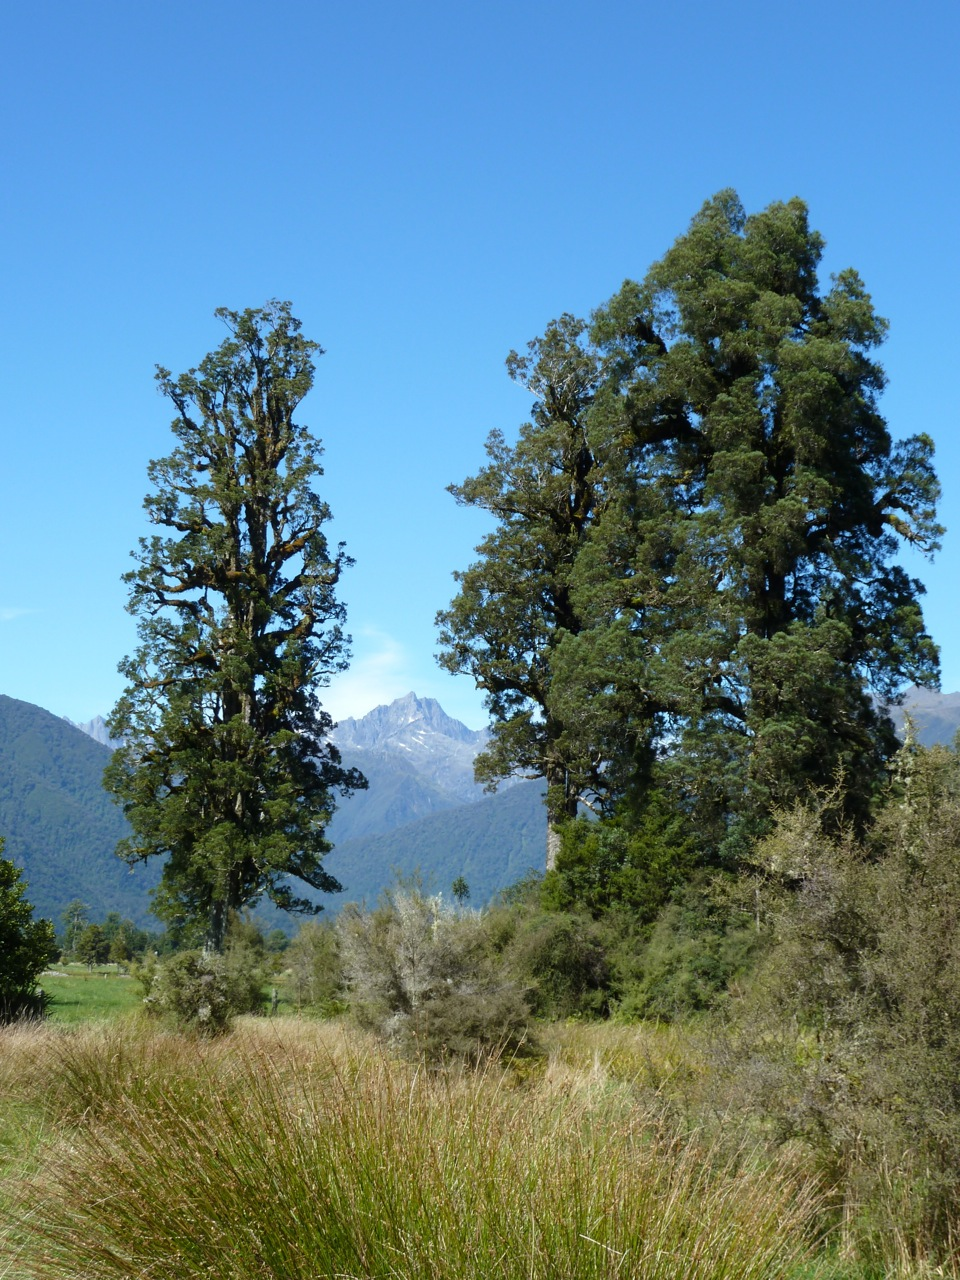
\includegraphics[width=\linewidth]{img+txt/matheson_baum.jpg}
        \end{minipage}
        \hfill
        {\Large $\stackrel{?}{\leadsto}$}
        \hfill
        \begin{minipage}{.45\textwidth}
          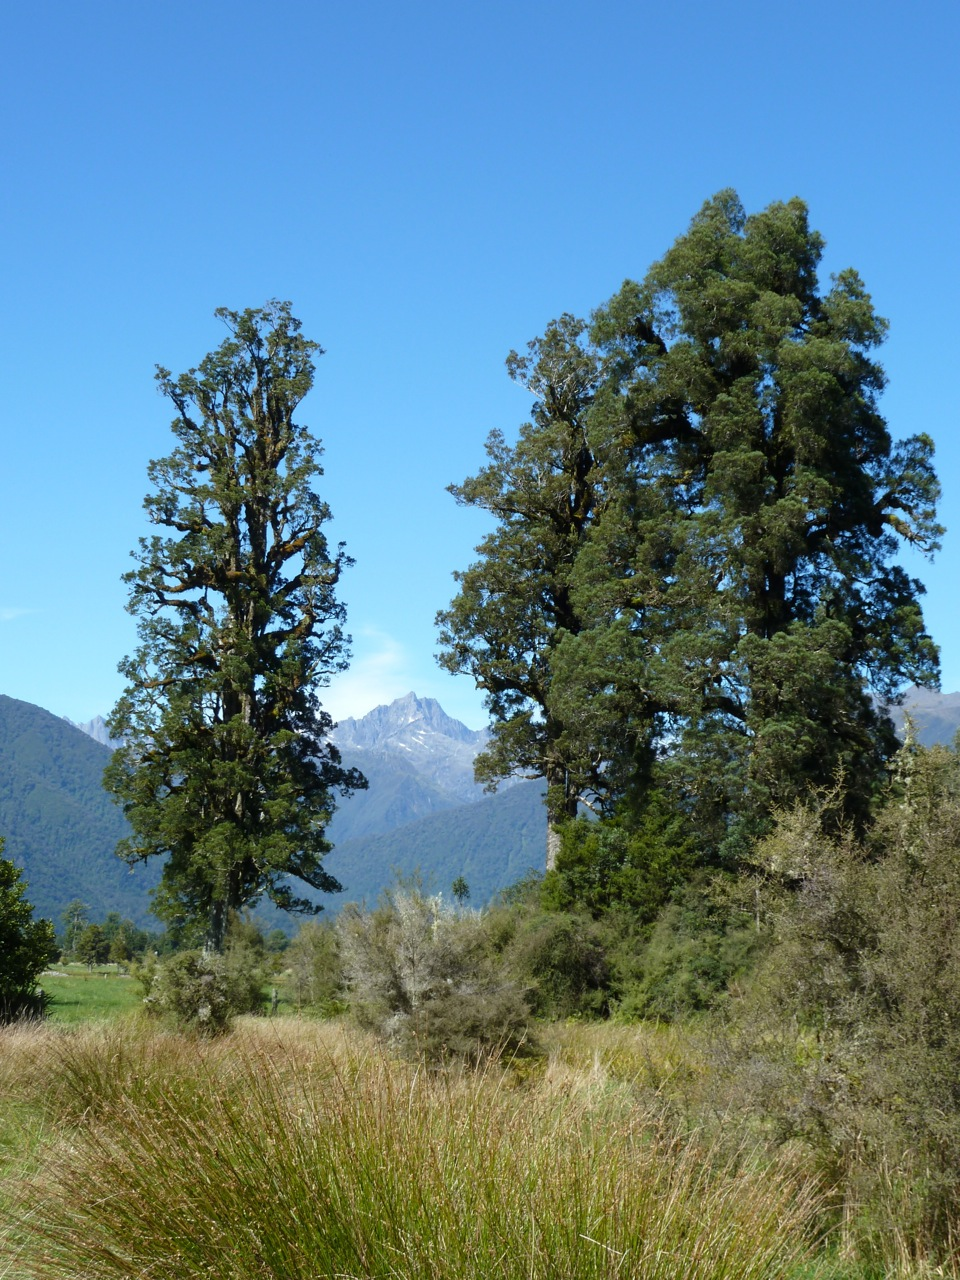
\includegraphics[width=\linewidth,angle=180]{img+txt/matheson_baum.jpg}
        \end{minipage}
      \end{center}

      \note{
        \textbf{16:00}
        
        \par
      }
    \end{frame}

  % ------------------------------------------------------------------------------------------
    \begin{frame}
      \frametitle{Top-down-Baumautomaten}

      \dots\ weisen der Wurzel einen Startzustand zu \\
      und arbeiten sich dann von oben nach unten zu den Blättern durch:

      \par\medskip
%      \uncover<2->{%
        \begin{definition}
          Ein \Bmph{nichtdet.\ Top-down-Automat auf endl.\ geord.\ Bäumen (\NETDBA)}\\
          ist ein Quadrupel $\Aut{A} = (Q,\Sigma,\Delta,I)$, wobei
          \begin{Itemize}
            \item
              $Q$ eine endliche nichtleere \Bmph{Zustandsmenge} ist,
            \item
              $\Sigma$ ein r-Alphabet ist,
            \item
              $\Delta$ eine Menge von \Bmph{Überführungsregeln} der Form
              \[
                  (a,q) \to (q_1,\dots,q_m)
              \]
              ist mit $m \geqslant 0$,\quad $a \in \Sigma_m$,\quad $q,q_1,\dots,q_m \in Q$,\quad und
            \item
              $I \subseteq Q$ die Menge der \Bmph{Anfangszustände} ist.
          \end{Itemize}%
          \label{def:NETDBA}%
          \vspace*{-2mm}
        \end{definition}
%      }


      \note{
        \textbf{16:00}
        
        \par
      }
    \end{frame}

    % ------------------------------------------------------------------------------------------
    \begin{frame}
      \frametitle{Berechnungen, Akzeptanz und erkannte Sprache}
      \begin{Definition}
        Sei $\Aut{A} = (Q,\Sigma,\Delta,I)$ ein NETDBA und $T=(P,t)$ ein $\Sigma$-Baum.
        \begin{Itemize}
          \item
            \Bmph{Run} von \Aut{A} auf $T$
            ist eine Fkt.\ $r : P \to Q$ mit:
            \begin{Itemize}
              \item
                $r(\varepsilon) \in I$
              \item<2->
                Wenn $t(p) = a \in \Sigma_m$ $(m \geqslant 1)$ und $r(p) = q$ \\
                und wenn $r(p1) = q_1$,\quad \dots,\quad $r(pm) = q_m$,
                \par\smallskip
                \uncover<3->{%
                  dann gibt es eine Regel $(a,q) \to (q_1,\dots,q_m) \in \Delta$.%
                }
              \item<4->
                Wenn $t(p) = a \in \Sigma_0$ und $r(p) = q$, dann $(a,q) \to () \in \Delta$.
            \end{Itemize}
%           \item
%             Ein Run $r$ von \Aut{A} auf $T$ ist \Bmph{erfolgreich}, wenn $r(\varepsilon) \in F$.
          \item<5->
            \Aut{A} \Bmph{akzeptiert} $T$, wenn es einen Run von \Aut{A} auf $T$ \Emph{gibt}.
          \item<6->
            Die von \Aut{A} \Bmph{erkannte Sprache} ist
            \par
            $L(\Aut{A}) = \{T \text{~über~} \Sigma \mid \Aut{A} \text{~akzeptiert~} T\}$.
        \end{Itemize}
      \end{Definition}

      \par\bigskip
      \uncover<7->{%
        \Emph{Beachte:}
        Keine Endzustände nötig -- die Regeln in $\Delta$ müssen nur erlauben, von der Wurzel bis zu allen Blättern "`durchzukommen"'.
      }

      \note{
        \textbf{16:03}
        
        \par
      }
    \end{frame}

    % ------------------------------------------------------------------------------------------
    \begin{frame}
      \frametitle{Beispiel 1}

      \begin{Itemize}
        \item
          Sei $\Sigma = \{a/2,~ b/0,~ c/0\}$ und

          \begin{minipage}{\linewidth}
            \begin{exampleblock}{}
              $\Aut{A} = (\{q_0,q_1,q_2,q_x\},~ \Sigma,~ \Delta,~ \{q_0\})$ mit
              \begin{alignat*}{4}
                \Delta & = \{   ~& (a,q_0) & \to (q_1,q_1), & \quad (b,q_2) & \to (), & \\
                       &         & (a,q_1) & \to (q_2,q_2), & \quad (c,q_2) & \to (), & \\
                       &         & (a,q_0) & \to (q_x,q_x)  &               &         &~\}
              \end{alignat*}
            \end{exampleblock}
          \end{minipage}


          \par\smallskip
        \item<2->
          Dann gibt es auf dem Baum
          \begin{center}
            \begin{minipage}{.21\textwidth}
              \Fig{31}
            \end{minipage}
            ~
            nur 1 Run:
            ~
            \uncover<3->{%
              \begin{minipage}{.21\textwidth}
                \Fig{34}
              \end{minipage}%
            }
            \uncover<4->{%
              ~
              \begin{minipage}{.255\textwidth}
                $\left(\raisebox{-8mm}{\Fig{35}}\right)$
              \end{minipage}%
            }
          \end{center}
          \par\bigskip
        \item<5->
          $L(\Aut{A}) =$
          \only<5|handout:0>{?}%
          \only<6->{$\{T \text{~über~} \Sigma \mid \text{alle Pfade in $T$ haben Länge 2}\}$}
%           \par\bigskip
%         \item<7->
%           \Bmph{Anmerkung:} Da $\Sigma$ nur $./2$ und $./0$ enthält:
%           \[
%             L(\Aut{A}) = \{T \text{~über~} \Sigma \mid T \text{~ist vollst.\ Binärbaum der Tiefe 2}\}
%           \]
%           \vspace*{-18.26pt}
      \end{Itemize}

      \note{
        \textbf{16:07}
        
        \par
      }
    \end{frame}

    % ------------------------------------------------------------------------------------------
    \begin{frame}
      \frametitle{Beispiel 2}

      Sei $\Sigma = \{a/2,~ b/1,~ c/0,~ d/0\}$.\quad Welcher NETDBA erkennt
      \par\smallskip
      $L_{\text{cd}} = \{T \text{~über~} \Sigma \mid \text{~jedes $c$-Blatt hat ein rechtes $d$-Geschwister}\}$?
% 
%       \par\smallskip
      \uncover<2->{%
        \begin{minipage}{\linewidth}
          \begin{exampleblock}{}
            NETDBA\quad $\Aut{A} = (\{q_0,q_c,q_d\},\Sigma,\Delta,\{q_0\})$ mit
            \vspace*{-1mm}
            \begin{alignat*}{4}
            \Delta & = \{~& (a,q_0) & \to (q_0,q_0), & \quad b(q_0) & \to q_0, & \quad (c,q_c) & \to (), \\
                   &      & (a,q_0) & \to (q_c,q_d), &              &          &       (d,q_d) & \to (), \\
                   &      &         &                &              &          &       (d,q_0) & \to ()~\}
            \end{alignat*}
            \vspace*{-7.7mm}
          \end{exampleblock}
        \end{minipage}

%         \par\smallskip
%         \begin{small}
%           \dgra{$(a,q_0) \to (q_d,q_d)$ überflüssig: $(a,q_0) \to (q_0,q_0)$ und $(d,q_0) \to ()$}
%           \par
%         \end{small}
      }

      \par\medskip
      \uncover<3->{%
        \begin{minipage}{\linewidth}
          \begin{exampleblock}{}
            \Bmph{Vergleiche} mit dem NEBA\quad  $\Aut{A} = (\{q_c,q_d,q_f\},\Sigma,\Delta,\{q_f\})$ mit
            \vspace*{-1mm}
            \begin{alignat*}{5}
              \Delta & = \{   ~& a(q_f,q_f) & \to q_f,  & \quad b(q_f) & \to q_f,  & \quad c & \to q_c, & \\
                     & \qquad ~& a(q_c,q_d) & \to q_f,  &              &           &       d & \to q_d, & \\
                     & \qquad ~&            &           &              &           &       d & \to q_f  &~\}
            \end{alignat*}
            \vspace*{-7.7mm}
          \end{exampleblock}
        \end{minipage}
      }

      \par\medskip
      \uncover<4->{%
        Was sagt uns das über das Verhältnis NETDBAs : NEBAs?
      }

      \note{
        \textbf{16:11}
        
        \par
      }
    \end{frame}

  \newcommand{\upa}{\ensuremath{\mathord{\uparrow}\!\!\!}}
  % ------------------------------------------------------------------------------------------
    \begin{frame}
      \frametitle{NETDBAs vs.\ NEBAs}
      
      \Bmph{NETDBAs und NEBAs sind gleichmächtig!}

      \par\smallskip
      \begin{Satz}
        $\{L(\Aut{A}) \mid \Aut{A} \text{~ist ein NETDBA}\}
        \quad=\quad
        \{L(\Aut{A}) \mid \Aut{A} \text{~ist ein NEBA}\}$.
      \end{Satz}

      \par\smallskip
      \uncover<2->{%
        \Bmph{Beweis.}~
        Sei $\Amc = (Q,\Sigma,\Delta,I)$ ein NE\Emph{TD}BA.
        
        \par\smallskip
        Konstruieren NEBA $\Amc^{\upa} = (Q,\Sigma,\Delta^{\upa},F^{\upa})$ mit:
        %
        \begin{align*}
          \Delta^{\upa} & ~=~ \{a(q_1,\dots,q_m) \to q) ~\mid~ (a,q) \to (q_1,\dots,q_m) \in \Delta\} \\
          F^{\upa}      & ~=~ I
        \end{align*}
      }    
    
      \par\vspace*{-\baselineskip}
      \uncover<3->{%
        Dann ist jeder Run von \Amc auf einem $\Sigma$-Baum $T$ \\
        auch ein \Emph{erfolgreicher} Run von $\Amc^{\upa}$ auf $T$ \\
        und umgekehrt.
      }
    
      \par\medskip
      \uncover<4->{%
        Daraus folgt $L(\Amc^{\upa}) = L(\Amc)$.
      }
    
      \par\medskip
      \uncover<5->{%
        Rückrichtung analog.
        \qed
      }
%%%    
%%%
%%%      \par\bigskip
%%%      Beweis: siehe Übungsblatt 2
%%%      % TODO: Ist das gut? Beweis ist nicht besonders anspruchsvoll und kann in Meghyns Skript nachgelesen werden.

      \note{
        \textbf{16:15 $\to$ bis 16:20}
        
        \par
      }
    \end{frame}

  \newcommand{\empha}[3]{%
    \only<#1|handout:0>{\rule[-10pt]{0pt}{1pt}#3}%
    \only<#2>{\rule[-10pt]{0pt}{1pt}\dred{\uwave{#3}}}%
  }
  % ------------------------------------------------------------------------------------------
    \begin{frame}
      \frametitle{Determinisierung von NETDBAs}
      
      \Bmph{Erinnerung an Beispiel 2:}\quad Sei $\Sigma = \{a/2,~ b/1,~ c/0,~ d/0\}$ und
      \par\smallskip
      $L_{\text{cd}} = \{T \text{~über~} \Sigma \mid \text{~jedes $c$-Blatt hat ein rechtes $d$-Geschwister}\}$.
% 
%       \par\smallskip
      \uncover<2->{%
        \begin{minipage}{\linewidth}
          \begin{exampleblock}{}
            NETDBA $\Aut{A} = (\{q_0,q_c,q_d\},\Sigma,\Delta,\{q_0\})$ mit
            \vspace*{-1mm}
  %           \begin{alignat*}{4}
  %             \Delta & = \{~& (a,q_0) & \to (q_0,q_0), & \quad b(q_0) & \to q_0, & \quad (c,q_c) & \to (), \\
  %                    &      & (a,q_0) & \to (q_c,q_d), &              &          &       (d,q_d) & \to (), \\
  %                    &      &         &                &              &          &       (d,q_0) & \to ()~\}
  %           \end{alignat*}
  %
  %            \begin{tikzpicture}
  %             \uncover<1->{%
  %               \node[inner sep=0pt]{%
  %                 bla%
  % %                 \begin{alignat*}{4}
  % %                   \Delta & = \{~& (a,q_0) & \to (q_0,q_0), & \quad b(q_0) & \to q_0, & \quad (c,q_c) & \to (), \\
  % %                         &      & (a,q_0) & \to (q_c,q_d), &              &          &       (d,q_d) & \to (), \\
  % %                         &      &         &                &              &          &       (d,q_0) & \to ()~\}
  % %                 \end{alignat*}
  %               };%
  %             }%
  %             \uncover<2->{\draw[draw=red,very thick]  (-0.33,-0.1) circle (7pt);}
  %           \end{tikzpicture} 
  %
  %           \begin{alignat*}{4}
  %             \Delta & = \{~& \empha{-1}{2-}{(a,q_0)}       & \to (q_0,q_0), & \quad b(q_0) & \to q_0, & \quad (c,q_c) & \to (), \\[-6pt]
  %                    &      & \empha{-1}{2-}{(a,q_0)}       & \to (q_c,q_d), &              &          &       (d,q_d) & \to (), \\[-6pt]
  %                    &      & \multicolumn{2}{c}{\only<2->{\dred{Nichtdet.!}}}  &                &              &          &       (d,q_0) & \to ()~\}
  %           \end{alignat*}
            \[
              \begin{array}{@{}r@{~}l@{~}r@{~}c@{~}l@{\quad}r@{~}c@{~}l@{\quad}r@{~}c@{~}l@{}}
                \Delta & = \{~& \empha{-2}{3-}{(a,q_0)} & \to & (q_0,q_0), & b(q_0) & \to & q_0, & (c,q_c) & \to & (), \\[-3pt]
                      &      & \empha{-2}{3-}{(a,q_0)} & \to & (q_c,q_d), &        &     &      & (d,q_d) & \to & (), \\[-3pt]
                      &      & \multicolumn{5}{l}{\only<3->{\dred{\text{{\small ~\raisebox{2pt}{$\blacktriangle$}~Nichtdeterminismus!}}}}}&& (d,q_0) & \to & ()~\}
              \end{array}
            \]
  %           \vspace*{-7.7mm}
          \end{exampleblock}
        \end{minipage}
        
%         \par\smallskip
%         \begin{minipage}{\linewidth}
%           \begin{exampleblock}{}
%             NEBA $\Aut{A} = (\{q_c,q_d,q_f\},\Sigma,\Delta,\{q_f\})$ mit
%             \vspace*{-1mm}
%             \begin{alignat*}{5}
%               \Delta & = \{   ~& a(q_f,q_f) & \to q_f,  & \quad b(q_f) & \to q_f,  & \quad c & \to q_c, & \\
%                      & \qquad ~& a(q_c,q_d) & \to q_f,  &              &           &       d & \to q_d, & \\
%                      & \qquad ~&            &           &              &           &       d & \to q_f  &~\}
%             \end{alignat*}
%             \vspace*{-7.7mm}
%           \end{exampleblock}
%         \end{minipage}%
      }

      \par\bigskip
      \uncover<4->{%
        Wir wissen ja, wie man Nichtdeterminismus "`loswird"'.
        \quad
        \Emph{Oder?}%
      }

      \note{
        \textbf{16:20}
        
        \parI
        Schauen wir uns auch hier noch die deterministische Variante von Top-down-Baumautomaten an.
        
        \par
      }
    \end{frame}

  % ------------------------------------------------------------------------------------------
    \begin{frame}
      \frametitle{Determinisierung von NETDBAs?}

      \Bmph{Betrachte}
      \begin{Itemize}
        \item
          $\Sigma = \{a/2,~ b/0,~ c/0\}$\quad und
        \item
          die erkennbare Baumsprache $L = \{a(bc), a(cb)\}$.\\
          \hfill{\footnotesize \emph{(denke an die alternative Schreibweise von Folie \ref{frame:baumbeispiel})}}
      \end{Itemize}

      \par\smallskip
      \Emph{Frage:}~ Welcher DETDBA erkennt $L$\,?

      \par\bigskip
      \uncover<2->{%
        \Gmph{Anwort:}~ Keiner!
        
        \par\smallskip
        \begin{Lemma}
          $L$ wird von keinem DETDBA erkannt.
        \end{Lemma}

        \par\smallskip
        Beweis: siehe Tafel. \Tafel
      }
      
      \par\medskip
      \uncover<3->{%
        \begin{korollar}
          Es gibt erkennbare Baumsprachen,\\
          die nicht von einem DETDBA erkannt werden.
        \end{korollar}

      }

      \note{
        \textbf{16:23 bis 16:30}
        
        \parI
        Konsequenz: DETDBAs sind schwächer als DEBAs (und NE(TD)BAs); \\
        NEBAs bleiben das Standardmodell!
        
        \par
      }
    \end{frame}

%%%  }

  % ==============================================================================================
  % ==============================================================================================
  \section[Abschlusseig.]{Abschlusseigenschaften}

%%%  \mysectioncontent{%
    % ------------------------------------------------------------------------------------------
    \begin{frame}
      \frametitle{Operationen auf Baumsprachen}

      Zur Erinnerung: die Menge der erkennbaren Baumsprachen heißt\\
      abgeschlossen unter \dots
      \begin{Itemize}
        \item
          \Bmph{Vereinigung}, falls gilt:
          \par\smallskip
          Falls $L_1,L_2$ erkennbar, so auch $L_1 \cup L_2$.
        \item
          \Bmph{Komplement}, falls gilt:
          \par\smallskip
          Falls $L$ erkennbar, so auch $\overline{L}$.
        \item
          \Bmph{Schnitt}, falls gilt:
          \par\smallskip
          Falls $L_1,L_2$ erkennbar, so auch $L_1 \cap L_2$.
      \end{Itemize}

      \par\smallskip
      \begin{alertblock}<2->{Quiz}
%       \uncover<2->{%
%         \Bmph{Quiz:}
        Unter welchen Operationen sind die NEBA-erkennbaren Sprachen abgeschlossen?
        \par\vspace*{-\baselineskip}
        \begin{center}
          \begin{tabular}{ll}
            Vereinigung? & \uncover<3-|handout:0>{\YES} \\
            Komplement?  & \uncover<4-|handout:0>{\YES} \\
            Schnitt?     & \uncover<5-|handout:0>{\YES}
          \end{tabular}
        \end{center}
      \end{alertblock}
%       }

      \note{
        \textbf{16:30}

        \par
      }
    \end{frame}

    % ------------------------------------------------------------------------------------------
    \begin{frame}
      \frametitle{Abgeschlossenheit}

      \begin{Satz}
        Die Menge der NEBA-erkennbaren Sprachen ist abgeschlossen unter den Operationen
        $\cup,\cap,\overline{\phantom{o}}$.
      \end{Satz}

      \par\bigskip
%      \uncover<2->{
        Direkte Konsequenz aus den folgenden Lemmata.
%      }


      \note{
        \textbf{16:33}

        \par
      }
    \end{frame}

    % ------------------------------------------------------------------------------------------
    \begin{frame}[t]
      \frametitle{Abgeschlossenheit unter Vereinigung}

      \begin{Lemma}
        Seien $\Aut{A}_1,\Aut{A}_2$ NEBAs über $\Sigma$.\\
        Dann gibt es einen NEBA $\Aut{A}_3$ mit $L(\Aut{A}_3) = L(\Aut{A}_1) \cup L(\Aut{A}_2)$.
        \label{lem:abgeschlossenheit_vereinigung}%
      \end{Lemma}

      \par\medskip
      \uncover<2->{
        \Bmph{Beweis.}~ analog zu NEAs:
        \par\medskip
        Seien $\Aut{A}_i = (Q_i, \Sigma, \Delta_i, F_i)$ für $i=1,2$.
        \par
        O.\,B.\,d.\,A.\ gelte $Q_1 \cap Q_2 = \emptyset$.
        \par\medskip
        Konstruieren $\Aut{A}_3 = (Q_3, \Sigma, \Delta_3, F_3)$ wie folgt.%
      }
      %
      \uncover<3->{
        \begin{Itemize}
          \item
            $Q_3 = Q_1 \cup Q_2$
          \item
            $\Delta_3 = \Delta_1 \cup \Delta_2$
          \item
            $F_3 = F_1 \cup F_2$
        \end{Itemize}
      }

      \par\smallskip
      \uncover<4->{
        Dann gilt:~ $L(\Aut{A}_3) = L(\Aut{A}_1) \cup L(\Aut{A}_2)$
        \qed%
      }


      \note{
        \textbf{16:34 bis 16:38}

        \par\medskip
        \textbf{Letzte Zeile:} \\
        Zeige:~ jeder Run von $\Amc$ auf $T$ entspricht einem Run von $\Amc_1$ oder $\Amc_2$,\\
        und umgekehrt.
        
%        \par\medskip
%        \textbf{Fragebogen F.\,1}~ ab nächste Folie für Euch zum Festhalten der Hauptideen
%        
        \par
      }
    \end{frame}

    % ------------------------------------------------------------------------------------------
    \begin{frame}[t]
      \frametitle{Abgeschlossenheit unter Komplement}

      \begin{Lemma}
        Sei $\Aut{A}$ ein NEBA über $\Sigma$.\\
        Dann gibt es einen NEBA $\Aut{A}^c$ mit $L(\Aut{A}^c) = \overline{L(\Aut{A})}$.
      \end{Lemma}

      \par\medskip
      \uncover<2->{
        \Bmph{Beweis:}~ analog zu NEAs:
        \begin{Itemize}
          \item
            Umwandlung in DEBA
          \item
            Vertauschen von akzeptierenden und nicht-akz.\ Zuständen
        \end{Itemize}
      }

      \par\medskip
      \uncover<3->{
        Sei $\Amc = (Q,\Sigma,\Delta,F)$.
        \par\medskip
        Nach Satz~\ref{thm:potenzmengenkonstruktion} gibt es \Emph{D}EBA
        $\Amc^d = (Q^d,\Sigma,\Delta^d,F^d)$
        mit $L(\Amc^d) = L(\Amc)$ und \Emph{genau einem} Run pro Eingabebaum.
      }

      \par\medskip
      \uncover<4->{
        Dann erkennt $\Aut{A}^c = (Q^d, \Sigma, \Delta^d, Q^d\setminus F^d)$ die Sprache $\overline{L(\Aut{A})}$.\qed%
      }

%       \par\bigskip
%       \uncover<3->{%
%         \centerline{$
%           \left(
%             \begin{array}{@{}l@{}}
%               \text{Jetzt erhält man Abgeschlossenheit unter $\cap$ auch mittels} \\
%               L_1 \cap L_2 = \overline{\overline{L_1} \cup \overline{L_2}}).
%             \end{array}
%           \right)
%         $}
%       }


      \note{
        \textbf{16:38 bis 16:40}

        \par
      }
    \end{frame}

    % ------------------------------------------------------------------------------------------
    \begin{frame}
      \frametitle{Abgeschlossenheit unter Schnitt}

      \begin{Lemma}
        Seien $\Aut{A}_1,\Aut{A}_2$ NEBAs über $\Sigma$.\\
        Dann gibt es einen NEBA $\Aut{A}_3$ mit $L(\Aut{A}_3) = L(\Aut{A}_1) \cap L(\Aut{A}_2)$.
        \label{lem:abgeschlossenheit_schnitt}%
      \end{Lemma}
      
      \par\medskip
      \dots folgt direkt aus der Abgeschlossenheit unter $\cup$ und $\overline{\phantom{o}}$:
      \[
        L_1 \cap L_2 = \overline{\overline{L_1} \cup \overline{L_2}}
      \]
      
      \par\bigskip
      \uncover<2->{%
        \begin{tabular}{@{}l@{~}l@{}}
          \Bmph{Alternative:} & Konstruktion des Produktautomaten wie für NEAs \\
                              & (vermeidet exponentielle ``Explosion'')
        \end{tabular}%
      }


      \note{
        \textbf{16:40}
        
        \par
      }
    \end{frame}

    % ------------------------------------------------------------------------------------------
    \begin{frame}
      \frametitle{Abgeschlossenheit unter Verkettungsoperationen}

      \Bmph{Randbemerkung:}

      \par %\smallskip
      Man kann
      Analoga zu $\cdot$ und ${}^*$ für Baumsprachen definieren:

      \par\bigskip
      Seien $L,L_1,L_2$ Baumsprachen.

      \par\medskip
      Bezeichne \Bmph{$\text{Con}(L)$} die Menge aller Kontexte, die man aus Bäumen in $L$ erhält, indem man ein Blattsymbol durch $x$ ersetzt.

      \begin{block}{}
        \begin{Itemize}
          \item
            $L_1L_2 = \{C[T] \mid T \in L_1,~ C \in \text{Con}(L_2)\}$
            \par\smallskip
          \item
            $L^* = \{C_1[C_2[\dots[C_n[T]]\dots]] \mid $\\[2pt]
            ~\hspace*{\fill}$T \in L,~ C_1,\dots,C_n \in \text{Con}(L),~ n \geqslant 0\}$
        \end{Itemize}
      \end{block}

      \par\bigskip
      Abgeschlossenheit unter $\cdot,{}^*$ kann man dann wie für NEAs zeigen, aber mit mehr technischem Aufwand (Eliminierung $\varepsilon$-Kanten \dots)


      \note{
        \textbf{16:41 bis 16:44;~ 5min Pause, 1min Puffer $\to$ 16:50}
        
        \par\medskip
        Beachte: Bäume sind nach Def. nichtleer. \\
        Deshalb schließt die Def. von $L^*$ den leeren Baum auch aus.
        \par
      }
    \end{frame}

%%%  }

  % ==============================================================================================
  % ==============================================================================================
  \section[Entscheid.-probl.]{Entscheidungsprobleme}

%%%  \mysectioncontent{%
    % ------------------------------------------------------------------------------------------
    \begin{frame}[t]
      \frametitle{Das Leerheitsproblem}
      
      \Bmph{Eingabe:}~ NEBA (oder DEBA) \Aut{A}

      \par\smallskip
      \Bmph{Frage:}~ Ist $L(\Aut{A}) = \emptyset$\,?
      
      \par\medskip
      \begin{tabular}{@{}l@{~~}l@{}}
%        d.\,h. & $\Bmph{$\text{LP}_\text{NEBA}$} = \{\Aut{A} \mid \Aut{A} \text{~NEBA,~} L(\Aut{A}) = \emptyset\}$, \\
%               & $\Bmph{$\text{LP}_\text{DEBA}$} = \{\Aut{A} \mid \Aut{A} \text{~DEBA,~} L(\Aut{A}) = \emptyset\}$
        d.\,h. & $\Bmph{$\text{LP}_\text{NEBA}$} = \{\Aut{A} \mid \Aut{A} \text{~NEBA,~} L(\Aut{A}) = \emptyset\}$
                 ~~~(analog für DEBAs)
      \end{tabular}
      
      \par\medskip
      \begin{Satz}<2->
        $\text{LP}_\text{NEBA}$ und $\text{LP}_\text{DEBA}$ sind entscheidbar
        und \PT-vollständig.
      \end{Satz}
      
      \par\medskip
      \uncover<3->{%
        \Bmph{Beweis.}
        %
        \begin{Itemize}
          \item
            Entscheidbarkeit in Polyzeit analog zu NEAs:\\
            prüfe, ob ein akz.\ Zustand erreichbar ist~ (nächste Folie)  %\Tafel
            \parI
          \item<4->
            \PT-Härte:\\
            Reduktion von "`Solvable Path Systems"' \\[2pt]
            \begin{small}
              ($\approx$ Erreichbarkeit in Hypergraphen mit ternärer Kantenrelation), \\
              siehe \cite[Exercise 1.19]{CDG+08}
              \par
            \end{small} 
%            \qed
        \end{Itemize}
      }      

      \note{
        \textbf{16:50}
        
        \par
      }
    \end{frame}
    
    % ------------------------------------------------------------------------------------------
    \begin{frame}
      \frametitle{Das Leerheitsproblem}
      
      \Bmph{Polynomialzeitalgorithmus:}
      \begin{Itemize}
        \item
          Berechne Menge der erreichbaren Zustände
        \item
          Prüfe, ob ein akzeptierender Zustand darin ist.
      \end{Itemize}
    
      \par\smallskip
      \uncover<2->{%
        Sei $\Amc = (Q,\Sigma,\Delta,F)$.
        \par\medskip
        Konstruieren Menge $R \subseteq Q$ wie folgt:
        %
        \begin{Itemize}
          \item
            $R := \{q \mid a \to q \in \Delta \text{~für ein~} a \in \Sigma_0\}$
          \item
            Wenn es $q_1,\dots,q_m \in R$ und $a \in \Sigma_m$ gibt mit $a(q_1,\dots,q_m) \to q \in \Delta$
            und $q \notin R$,~ dann $R := R \cup \{q\}$.
          \item
            Wiederhole letzten Schritt, bis sich $R$ nicht mehr ändert.
        \end{Itemize}
      }
    
      \par\smallskip
      \uncover<3->{%
        \begin{tabular}{@{}l@{~~}l@{}}
          \Bmph{Leicht zu sehen:}~
          & Berechnung endet nach $\leq |Q|$ vielen Schritten\\
          & $\leadsto$ $R$ ist in Polyzeit berechenbar.
        \end{tabular}
      }

      \par\medskip
      \uncover<4->{%
        \Bmph{Noch zu zeigen:}\quad
        $L(\Amc) = \emptyset$ ~gdw.~ $R \cap F = \emptyset$ \hfill\hfill \Tafel \qed
      }

      \note{
        \textbf{16:53 bis 17:18}
        
        \parI
        "`in Polyzeit:"'~ weil $R$ monoton wachsend und durch $Q$ beschränkt!
        
        \par\medskip
        Letzte Äquivalenz:~ erkannte Sprache leer ~gdw.~ kein akz.\ Zust. erreichbar

%        \par\medskip
%        \textbf{12:44~ Fragebogen F.\,2+3}\\
%        (F.\,2: wie F.\,1, aber für EP;~ F.\,3: Tabelle zum "`Aufsammeln"')
%        
%        \par\medskip
%        \textbf{5\,min Pause bis 12:49, dann Beweis bis 13:15}
        
        \par
      }
    \end{frame}

  % ------------------------------------------------------------------------------------------
    \begin{frame}
      \frametitle{Das Wortproblem alias Zugehörigkeitsproblem}
      
      \Bmph{Eingabe:}~ NEBA (oder DEBA) \Aut{A},~ Baum $T$ über $\Sigma$

      \par\smallskip
      \Bmph{Frage:}~ Ist $T \in L(\Aut{A})$\,?
      
      \par\medskip
      \begin{tabular}{@{}l@{~~}l@{}}
%        d.\,h. & $\Bmph{$\text{WP}_\text{NEBA}$} = \{(\Aut{A},T) \mid \Aut{A} \text{~NEBA,~} T \in L(\Aut{A})\}$, \\
%               & $\Bmph{$\text{WP}_\text{DEBA}$} = \{(\Aut{A},T) \mid \Aut{A} \text{~DEBA,~} T \in L(\Aut{A})\}$
        d.\,h. & $\Bmph{$\text{WP}_\text{NEBA}$} = \{(\Aut{A},T) \mid \Aut{A} \text{~NEBA,~} T \in L(\Aut{A})\}$
                 ~~~{\small (analog f.\ DEBAs)}
      \end{tabular}
      
      \par\medskip
      \begin{Satz}<2->
        $\text{WP}_\text{NEBA}$ und $\text{WP}_\text{DEBA}$ sind entscheidbar und in \PT.
      \end{Satz}
      
      \par\medskip
      \uncover<3->{%
        \Bmph{Beweis.}~ analog zu NEAs, per Reduktion zum LP:
        \par\medskip
        \hspace*{20mm} $T \in L(\Aut{A})$ ~gdw.~ $L(\Aut{A}) \cap L(\Aut{A}_T) \neq \emptyset$,
        \par\medskip
        wobei $\Amc_T$ ein DEBA mit $L(\Amc_T) = \{T\}$ ist (konstruiere selbst!)
        \qed
      }      
      
      \par\bigskip
      \uncover<4->{%
        $
          \left(~~
            \text{%
              \begin{tabular}{@{}l@{}}
                $\text{WP}_\text{NEBA}$ ist LOGCFL-vollständig.~ (zwischen \NL und \PT) \\[3pt]
                $\text{WP}_\text{DEBA}$ ist in LOG\Emph{D}CFL.~ (Genaue Komplexität ist offen!) \\[3pt]
                $\text{WP}_\text{DE\Emph{TD}BA}$ ist \LS-vollständig.
              \end{tabular}%
            }
          \right)
        $
      }      

      \note{
        \textbf{17:18 bis 17:22}

        \parI
        "`alias"':~ Bäume sind eben keine Wörter. Werde trotzdem weiter "`WP"' benutzen.
        
        \par\medskip
        LOGCFL:\\
        Probleme, die sich in logspace aufs Wortproblem für kfS reduzieren lassen
        
        \par\medskip
        LOGDCFL:\\
        dito, aber Red.\ auf \emph{determinist.} kfS (d.\,h.\ durch DPDA erkennbar)
        
        \par\medskip
        L ~$\subseteq$~ \begin{tabular}{@{}c@{}}LogDCFL\\[3pt]NL\end{tabular} ~$\subseteq$~ LogCFL ~$\subseteq$~ P
        
        \par
      }
    \end{frame}

    % ------------------------------------------------------------------------------------------
    \begin{frame}
      \frametitle{Das Äquivalenzproblem}
      
      \Bmph{Eingabe:}~ NEBAs (oder DEBAs) $\Aut{A}_1,\Aut{A}_2$

      \par\smallskip
      \Bmph{Frage:}~ Ist $L(\Aut{A}_1) = L(\Aut{A}_2)$\,?
      
      \par\medskip
      \begin{tabular}{@{}l@{~~}l@{}}
%        d.\,h. & $\Bmph{$\text{ÄP}_\text{NEBA}$} = \{(\Aut{A}_1,\Aut{A}_2) \mid \Aut{A}_1,\Aut{A}_2 \text{~NEBAs,~} L(\Aut{A}_1) = L(\Aut{A}_2)\}$, \\
%               & $\Bmph{$\text{ÄP}_\text{DEBA}$} = \{(\Aut{A}_1,\Aut{A}_2) \mid \Aut{A}_1,\Aut{A}_2 \text{~DEBAs,~} L(\Aut{A}_1) = L(\Aut{A}_2)\}$
        d.\,h. & $\Bmph{$\text{ÄP}_\text{NEBA}$} = \{(\Aut{A}_1,\Aut{A}_2) \mid \Aut{A}_1,\Aut{A}_2 \text{~NEBAs,~} L(\Aut{A}_1) = L(\Aut{A}_2)\}$
                 ~etc.
      \end{tabular}
      
      \par\medskip
      \begin{Satz}<2->
        %        Das Wortproblem für NEAs bzw.\ DEAs ist entscheidbar \\
        %        und \NL-vollständig.
        $\text{ÄP}_\text{NEBA}$ und $\text{ÄP}_\text{DEBA}$ sind entscheidbar.\\
        $\text{ÄP}_\text{NEBA}$ ist \EXP-vollständig;~ $\text{ÄP}_\text{DEBA}$ ist in \PT.
      \end{Satz}
      
      \par\medskip
      \uncover<3->{%
        \Bmph{Beweis.}
        %
        \begin{Itemize}
          \item
            Entscheidbarkeit analog zu NEAs, per Reduktion zum LP:\\
            \par\medskip
            \hspace*{10mm} $L(\Aut{A}_1) = L(\Aut{A}_2)$ ~gdw.~ $L(\Aut{A}_1) \vartriangle L(\Aut{A}_2) = \emptyset$
            \parI
          \item<4->
            obere Schranken:~ Automat für $L(\Aut{A}_1) \vartriangle L(\Aut{A}_2)$ ist exponentiell in
            der Größe der Eingabe-NEBAs /  polynomiell für DEBAs
          \item<5->
            \scalebox{.95}[1]{\EXP-Härte: Reduktion vom Universalitätsproblem (F.\,\ref{fra:universalitaet})}
%            \EXP-Härte: Reduktion vom Wortproblem für linear platzbeschränkte alternierende Turingmaschinen.
%          \item
%            siehe auch \cite[{CDG+08}
          \qed
        \end{Itemize}
      }      


      \note{
        \textbf{17:22 bis 17:25}

        \par\medskip
        $\vartriangle$ $=$ symmetrische Differenz zweier Mengen; \\
        ausdrückbar mittels $\cup,\cap,\overline{\cdot}$\quad $\leadsto$ Abschlusseigenschaften!
        
        \par\medskip
        Untere Schranke für DEBAs:~ weiß nicht \dots
      }
    \end{frame}

    % ------------------------------------------------------------------------------------------
    \begin{frame}
      \label{fra:universalitaet}
      \frametitle{Das Universalitätsproblem}
      
      \Bmph{Eingabe:}~ NEBA (oder DEBA) \Aut{A}

      \par\smallskip
      \Bmph{Frage:}~ Ist $L(\Aut{A}) = \calT(\Sigma)$\,?
      \hfill {\small $($\Bmph{$\calT(\Sigma)$} ${}= \{T \mid T \text{~ist ein $\Sigma$-Baum}\})$}
      
      \par\medskip
      \begin{tabular}{@{}l@{~~}l@{}}
%        d.\,h. & $\Bmph{$\text{UP}_\text{NEBA}$} = \{\Aut{A} \mid \Aut{A} \text{~NEBA,~} L(\Aut{A}) = \calT(\Sigma)\}$, \\
%               & $\Bmph{$\text{UP}_\text{DEBA}$} = \{\Aut{A} \mid \Aut{A} \text{~DEBA,~} L(\Aut{A}) = \calT(\Sigma)\}$
        d.\,h. & $\Bmph{$\text{UP}_\text{NEBA}$} = \{\Aut{A} \mid \Aut{A} \text{~NEBA,~} L(\Aut{A}) = \calT(\Sigma)\}$
                 ~~~{\small (analog f.\ DEBAs)}
      \end{tabular}
      
      \par\medskip
      \begin{Satz}<2->
        $\text{UP}_\text{NEBA}$ und $\text{UP}_\text{DEBA}$ sind entscheidbar.\\
        $\text{UP}_\text{NEBA}$ ist \EXP-vollständig;~ $\text{UP}_\text{DEBA}$ ist in \PT.
      \end{Satz}
      
      \par\medskip
      \uncover<3->{%
        \Bmph{Beweis:}~
        \begin{Itemize}
          \item
            Entscheidbarkeit \& obere Schranken per Red.\ zum ÄP:\\
            \par\medskip
            \hspace*{10mm} $L(\Aut{A}) = \calT(\Sigma)$ ~gdw.~ $L(\Aut{A}) = L(\Aut{A}_\Sigma)$,
            \par\medskip
            wobei $\Aut{A}_\Sigma$ DEBA mit $L(\Aut{A}_\Sigma) = \calT(\Sigma)$~ (konstruiere selbst!)
            \parI
          \item<4>
            \EXP-Härte: Red.\ vom WP für lin.\ platzbeschränkte alternierende TM
            (s.\,a.\ \cite[\S\,1.7]{CDG+08})
            \qed
        \end{Itemize}
      }

      \note{
        \textbf{17:25 bis 17:27}

        \par
      }
    \end{frame}

    \newlength{\sternchen}
    \settowidth{\sternchen}{${}^*$}
    \newcommand{\stNOst}{\hspace*{\sternchen}\NO{}${}^*$}
    % ------------------------------------------------------------------------------------------
    \begin{frame}
    \frametitle{Überblick Entscheidungsprobleme für NEBAs/DEBAs}
    
    %      \begin{center}
    \begin{tabular}{cccc}
      \hline\stab
              &               & für DEBAs         & für NEBAs         \\
      Problem & entscheidbar? & effizient lösbar? & effizient lösbar? \\
      \hline\stab
      LP      & \YES          & \YES              & \YES              \\
      WP      & \YES          & \YES              & \YES              \\
      ÄP      & \YES          & \YES              & \stNOst           \\
      UP      & \YES          & \YES              & \stNOst           \\
      \hline
    \end{tabular}
    
        \par\bigskip
        \begin{tabular}{@{}l@{\,}l@{}}
          ${}^*$ & nachweislich! (da $\EXP \neq \PT$)
        \end{tabular}
    %      \end{center}
    
      \note{
        \textbf{17:27 bis 17:29 $\leadsto$ 1\,min Reserve}
  
        \par
        Hier nochmal für Euch als Überblick
  
        \par\medskip
        Nächstes Mal: XML, Kapitel zuende
        
        \par\medskip
        Zum \textbf{Literaturverzeichnis} blättern
        
        \par
      }
    \end{frame}

%%%  }

  % ==============================================================================================
  % ==============================================================================================
  \section[\protect\emph{XML}]{\protect\emph{Anwendung: XML-Schemasprachen}}

%%%  \mysectioncontent{%
    % ------------------------------------------------------------------------------------------
    \begin{frame}
      \frametitle{Zur Erinnerung: semistrukturierte Daten}
      
      Daten werden in Entitäten (Einheiten) zusammengefasst
      \begin{Itemize}
        \item
          Markierung von Entitäten durch Tags
        \item
          Bildung von Hierarchien
        \item
          Gruppieren ähnlicher Entitäten
        \item
          Entitäten derselben Gruppe können \\
          verschiedene (oder keine) Attribute haben
        \item
          Reihenfolge der Attribute \emph{kann} eine Rolle spielen
          \par
          \uncover<2->{%
            {\small (Mengen oder Listen z.\,B.\ von Telefonnummern?)}%
          }
      \end{Itemize}
      
%       \begin{Beispiel}<2->
%         \begin{small}
%           \begin{ttfamily}
%             $\{$Name: $\{$VN: "Thomas", NN: "{}Schneider"$\}$, \\
%             ~Telnr: 64432, \\
%             ~Telnr: 43776243, \\
%             ~Email: "ts@informatik..."$\}$
%           \end{ttfamily}
%           \par
%         \end{small}
%       \end{Beispiel}
      \par\bigskip
      \uncover<2->{%
        \Gmph{Beispiel:}
        \quad
        \Bsp
      }

      \note{
        \uz{8:30}
        
        \par
      }
    \end{frame}

  % ------------------------------------------------------------------------------------------
    \begin{frame}
      \frametitle{Repräsentation im Baum}
      
      \hspace*{\fill}
      \Bsp
      \par\bigskip\bigskip
%       Repräsentation im Baum ist naheliegend:
      \begin{center}
        \Fig{1}
      \end{center}

      \note{
        \uz{8:32}
        
        \par
      }
    \end{frame}

  % ------------------------------------------------------------------------------------------
    \begin{frame}
      \frametitle{Größeres Bsp.: XML-Dokument für Konferenzprogramm}
      
      \begin{minipage}[b]{.6\textwidth}
        \begin{exampleblock}{}
          \includegraphics[width=\textwidth,trim=164 420 205 185,clip]{img+txt/tata230.pdf}
        \end{exampleblock}
      \end{minipage}
      \hfill
      \begin{minipage}[b]{.37\textwidth}
        \begin{footnotesize}
          aus \emph{Tree Automata Techniques and Applications}, S. 230
          \par
        \end{footnotesize}
      \end{minipage}


      \note{
        \uz{8:33}
        
        \par
      }
    \end{frame}

  % ------------------------------------------------------------------------------------------
    \begin{frame}
      \frametitle{Zugehöriger Baum}

      \begin{minipage}[b]{\textwidth}
        \begin{exampleblock}{}
          \includegraphics[width=\textwidth,trim=210 240 117 481,clip]{img+txt/tata230.pdf}
        \end{exampleblock}
      \end{minipage}
      \par
      \begin{footnotesize}
        \hspace*{\fill} aus \emph{Tree Automata Techniques and Applications}, S. 230
        \par
      \end{footnotesize}
      
      \par\bigskip
      \ddred{$\blacktriangleright$} \Emph{Ab jetzt:} wir beschreiben nur die Struktur, ignorieren die Daten

      \note{
        \uz{8:35}
        
        \par
      }
    \end{frame}


  % ------------------------------------------------------------------------------------------
    \begin{frame}
      \frametitle{Was ist ein gültiges Konferenzdokument?}

      \only<1|handout:0>{\Fig{41}}%
      \only<2->{\Fig{42}}
      \hspace*{1cm}
      \only<3|handout:0>{\Fig{43}}%
      \only<4->{\Fig{44}}
      
      

      \note{
        \uz{8:37}
        
        \par
      }
    \end{frame}

  % ------------------------------------------------------------------------------------------
    \begin{frame}
      \frametitle{Mögliche Anforderungen an gültige Konferenzdokumente}
      
      \begin{Itemize}
        \item
          Eine Konferenz kann in mehrere Blöcke (Tracks) geteilt sein.
        \item
          Jeder Block (oder die Konf. selbst, wenn sie keine Blöcke hat)\\
          ist in Sitzungen aufgeteilt.
        \item
          Jede Sitzung hat einen oder mehrere Vorträge.
        \item
          Jede Sitzung wird von einer Person geleitet (Chair).
        \item
          Jeder Vortrag hat einen Titel und
          \begin{Itemize}
            \item
              Autor\_innen (falls es sich um einen Konferenzbeitrag handelt)
            \item
              oder Vortragende\_n (falls es ein eingeladener Vortrag ist).
          \end{Itemize}
        \item
          Zwischen den Sitzungen kann es Pausen geben.
      \end{Itemize}


      \note{
        \uz{8:38}
        
        \par
      }
    \end{frame}

  % ------------------------------------------------------------------------------------------
    \begin{frame}
      \frametitle{Gültige Dokumente als Baumsprachen!}

      Die gelisteten Anforderungen beschreiben eine \Bmph{Baumsprache}\\
      über dem Alphabet $\{\texttt{conference},\texttt{track},\texttt{session},\dots\}$.

      \par\bigskip
      Eine solche Beschreibung wird auch \Bmph{Schema} genannt.

      \par\bigskip
      Ein Dokument ist \Bmph{gültig} für ein Schema,\\
      wenn sein Baum zur Baumsprache des Schemas gehört.

      \par\bigskip
      \uncover<2->{%
        \Emph{Ziele dieses Abschnitts}
        \begin{alertblock}{}
          \begin{Itemize}
            \item
              Vorstellen von XML-Schemasprachen
            \item
              Diskutieren von Verbindungen zur Automatentheorie
            \item
              Untersuchen der Ausdrucksstärke von Schemasprachen
            \item
              und ihre \Emph{Entscheidungsprobleme}
          \end{Itemize}  
        \end{alertblock}
      }


      \note{
        \uz{8:40}
        
        \par
      }
    \end{frame}

  % ------------------------------------------------------------------------------------------
    \begin{frame}
      \frametitle{Entscheidungsprobleme für XML-Schemasprachen}

      Die bekannten Entscheidungsprobleme
      entsprechen natürlichen Fragen für XML-Dokumente und -Schemasprachen:

%       \par\smallskip
%       \begin{Itemize}
%         \item<1->
%           \Bmph{Zugehörigkeitsproblem}
%           \par\smallskip
%           Ist ein gegebenes Dokument gültig für ein gegebenes Schema?
%           \par\smallskip
%           \begin{small}
%             (im Bsp.: erfüllt ein gegebenes Konf.-dokument die Anforderungen?)
%             \par
%           \end{small}
%           \par\smallskip
%         \item<2->
%           \Bmph{Leerheitsproblem}
%           \par\smallskip
%           Gibt es für ein gegebenes Schema gültige Dokumente?
%           \par\smallskip
%           \begin{small}
%             (Enthält das gegebene Schema keinen "`Widerspruch"'?)
%             \par
%           \end{small}
%           \par\smallskip
%         \item<3->
%           \Bmph{Äquivalenzproblem}
%           \par\smallskip
%           Haben zwei Schemata dieselben gültigen Dokumente?
%           \par\smallskip
%           \begin{small}
%             (Wichtig bei der Vereinfachung von Schemata:
%             Ist das Resultat der Vereinfachung äquivalent zum ursprünglichen Schema?)
%             \par
%           \end{small}
%           \par\smallskip
%       \end{Itemize}

      \par\bigskip
      \Bmph{Zugehörigkeitsproblem}
      \par\smallskip
      Ist ein gegebenes Dokument gültig für ein gegebenes Schema?
      \par\smallskip
      \begin{small}
        (im Bsp.: erfüllt ein gegebenes Konf.-dokument die Anforderungen?)
        \par
      \end{small}

      \par\bigskip
      \uncover<2->{%
        \Bmph{Leerheitsproblem}
        \par\smallskip
        Gibt es für ein gegebenes Schema gültige Dokumente?
        \par\smallskip
        \begin{small}
          (Enthält das gegebene Schema keinen "`Widerspruch"'?)
          \par
        \end{small}
      }

      \par\bigskip
      \uncover<3->{%
        \Bmph{Äquivalenzproblem}
        \par\smallskip
        Haben zwei Schemata dieselben gültigen Dokumente?
        \par\smallskip
        \begin{small}
          (Wichtig bei der Vereinfachung von Schemata)
          \par
        \end{small}
      }

      \note{
        \uz{8:42}
        
        \parI
        Zum ÄP, "`Vereinfachung von Schemata"': \\
        Ist das Resultat der Vereinfachung äquivalent zum ursprünglichen Schema?

        \par
      }
    \end{frame}

  % ------------------------------------------------------------------------------------------
    \begin{frame}
      \frametitle{Dokumenttypdefinitionen (DTDs)}

      DTDs sind ein Standard zur Beschreibung gültiger Dokumente

      \par\bigskip
      Eine DTD ist eine kontextfreie Grammatik (kfG),\\
      deren rechte Regelseiten reguläre Ausdrücke enthalten können

      \par\bigskip
      Ableitungsbäume der kfG bilden die Baumsprache,\\
      die durch die DTD bestimmt wird

      \note{
        \uz{8:44}
        
        \par
      }
    \end{frame}

  % ------------------------------------------------------------------------------------------
    \begin{frame}
      \frametitle{Beispiel-DTD für Konferenzdokumente}
      
%       \begin{exampleblock}{}
%         \includegraphics[width=\textwidth,trim=150 486 102 249,clip]{img+txt/tata232.pdf}
%       \end{exampleblock}
% 
      \begin{exampleblock}{}
        \begin{small}
          \begin{ttfamily}
            <!DOCTYPE CONFERENCE [ \\
            ~~<!ELEMENT conference~(track+|(session,break?)+)>        \\
            ~~<!ELEMENT track~~~~~~((session,break?)+)>               \\
            ~~<!ELEMENT session~~~~(chair,talk+)>                     \\
            ~~<!ELEMENT talk~~~~~~~((title,authors)|(title,speaker))> \\
            ~~<!ELEMENT chair~~~~~~(\#PCDATA)>                        \\
            ~~<!ELEMENT break~~~~~~(\#PCDATA)>                        \\
            ~~<!ELEMENT title~~~~~~(\#PCDATA)>                        \\
            ~~<!ELEMENT authors~~~~(\#PCDATA)>                        \\
            ~~<!ELEMENT speaker~~~~(\#PCDATA)>                        \\
          \end{ttfamily}
          \texttt{]> \hspace*{\fill} ,} $\hat=$ Verkettung
        \end{small}
      \end{exampleblock}

      \par\medskip
      \uncover<2->{%
        Beschreibt Bäume, in denen z.\,B.\ jeder \texttt{conference}-Knoten
        \begin{Itemize}
%           \item
%             \only<2|handout:0>{ein oder mehrere \texttt{track}-Kinder hat oder}%
%             \only<3->{\Emph{ein oder mehrere} \texttt{track}-\Emph{Kinder} hat oder\quad \mbox{\Emph{$\leadsto$ \uwave{beliebige Stelligkeit!}}\hspace*{-20mm}}}
%           \item
%             \only<2|handout:0>{ein oder mehrere \texttt{session}-Kinder hat,\\}%
%             \only<3->{\Emph{ein oder mehrere} \texttt{session}-\Emph{Kinder} hat,\\}%
%             zwischen denen einzelne \texttt{break}-Geschwister stehen dürfen
%
%           \item
%             ein oder mehrere \texttt{track}-Kinder hat oder\quad \mbox{\Emph{$\leadsto$ \uwave{beliebige Stelligkeit!}}\hspace*{-20mm}}
%           \item
%             ein oder mehrere \texttt{session}-Kinder hat, \\
%             zwischen denen einzelne \texttt{break}-Geschwister stehen dürfen
%
          \item
            \only<-2|handout:0>{ein oder mehrere \texttt{track}-Kinder hat oder\quad \mbox{\raisebox{-3mm}{\strut}}}%
            \only<3->{\uwave{ein oder mehrere} \texttt{track}-Kinder hat oder\quad \mbox{\raisebox{-3mm}{\strut\Emph{$\leadsto$ \uwave{beliebige Stelligkeit!}}\hspace*{-20mm}}}}
          \item
            \vspace*{-3mm}%
            \only<-2|handout:0>{ein oder mehrere \texttt{session}-Kinder hat,\\}%
            \only<3->{\uwave{ein oder mehrere} \texttt{session}-Kinder hat,\\}%
            zwischen denen einzelne \texttt{break}-Geschwister stehen dürfen
        \end{Itemize}
      }

      \note{
        \uz{8:45}
        
        \par
      }
    \end{frame}

  % ------------------------------------------------------------------------------------------
    \begin{frame}
      \frametitle{Wir brauchen Symbole mit beliebiger Stelligkeit!}
      
        \Bmph{Erweitern unser r-Alphabet:}
        \begin{Itemize}
          \item
            $U$: Menge von \Bmph{Symbolen ohne Stelligkeit}
          \item
            $\Sigma = U ~\cup~ \bigcup_{i\geqslant 0} \Sigma_i$
        \end{Itemize}

        \par\bigskip
        \uncover<2->{%
          \begin{block}{}
            \Bmph{Endlicher geordneter Baum} $T=(P,t)$ über $\Sigma$:
            \begin{Itemize}
              \item
                $P \subseteq \mathbb{N}_+^*$ nichtleere endl.\ präfix-abgeschlossene Menge
              \item
                $t: P \to \Sigma$ Funktion mit
                \begin{Enumerate}
                  \item
                    Wenn $t(p) \in \Sigma_m$, dann $\{j \mid pj \in P\} = \{1,\dots,m\}$.
                  \item
                    Wenn $t(p) \in U$, dann $\{j \mid pj \in P\} = \{1,\dots,k\}$\\
                    \hfill für ein $k \geqslant 0$.
                \end{Enumerate}
            \end{Itemize}
          \end{block}
        }


        \par\bigskip
        \uncover<3->{%
          \Bmph{Beschränken uns auf den Fall ohne Stelligkeit (o.\,S.):}~
%           \par\smallskip
          $
            \Sigma = U
          $%
        }

      \note{
        \uz{8:48}
        
        \par
      }
    \end{frame}

  % ------------------------------------------------------------------------------------------
    \begin{frame}
      \frametitle{Weitere Begriffe}
      
      \begin{Itemize}
        \item
          \Bmph{Höhe, Tiefe, Teilbaum}: wie für Bäume mit Stelligkeit
        \item
          \begin{tabular}[t]{@{}ll@{}}
            $a(T_1\cdots T_n)$: & Baum mit $a$ in Wurzel und \\
                                & Teilbäumen $T_1,\dots,T_n$ direkt darunter
          \end{tabular}
        \item
          \begin{tabular}[t]{@{}l@{~~}l@{}}
            \Bmph{Hecke (Hedge):} & Folge $T_1\cdots T_n$ von Bäumen \\ %o.\,S.\\
                                  & leere Hecke: \Bmph{$\varepsilon$}
          \end{tabular}
        \item
          \Bmph{$H(\Sigma)$:}~ Menge aller Hecken über $\Sigma$
      \end{Itemize}
      
      \par\smallskip
      \uncover<2->{%
        \begin{block}{}
          \Bmph{$\leadsto$ induktive Charakterisierung von Bäumen:} %o.\,S.:}
          \begin{Itemize}
            \item
%              Jede Folge von Bäumen o.\,S.\ ist eine Hecke. %\\
              Jede Folge von Bäumen ist eine Hecke. %\\
%              {\small (Das schließt die leere Folge ein.)}
            \item
              Wenn $h$ eine Hecke und $a \in \Sigma$ ein Symbol ist,\\
              dann ist $a(h)$ ein Baum %o.\,S.\
%              \hfill
%              $\blacktriangleleft\!$~ Bsp.: s.\ Tafel \Tafel
          \end{Itemize}
        \end{block}

        \par\medskip
        $h=\varepsilon$\quad $\leadsto$\quad schreiben $a$ statt $a(\varepsilon)$
      }

      \note{
        \uz{8:50}
        
        \par
      }
    \end{frame}
    
    % ------------------------------------------------------------------------------------------
    \begin{frame}
      \frametitle{Beispiele für Hecken und Bäume}

      Sei $\Sigma = \{a,b,c\}$.
      
      \par\bigskip
      $\varepsilon$ ist eine Hecke
      \par\smallskip
      \Bmph{$\leadsto$} $a = a()$ ist ein Baum
      \par\smallskip
      \Bmph{$\leadsto$} $aa$ ist eine Hecke
      \par\smallskip
      \Bmph{$\leadsto$} $b(aa)$ ist ein Baum
      \par\smallskip
      \Bmph{$\leadsto$} $ab(aa)c$ ist eine Hecke
      \par\smallskip
      \Bmph{$\leadsto$} $a(ab(aa)c)$ ist ein Baum
      \Tafel
      
      \par\bigskip
      \uncover<2->{%
        $(a(c(b)cb(ab))$ ist ein Baum
        \TafelForts
      }

      \note{
        \uz{8:53 bis 8:58}
        
        \par
      }
    \end{frame}

  % ------------------------------------------------------------------------------------------
    \begin{frame}
      \frametitle{Heckenautomaten}

      \dots sind Bottom-up-Automaten auf Bäumen ohne Stelligkeit %o.\,S.\
      
      \par\medskip
      Können sie analog zu NEBAs definiert werden?
      
      \uncover<2->{%
        \begin{Itemize}
          \item[]
            \Emph{Nein:}
            Weil Stelligkeit von $a \in \Sigma$ nicht festgelegt ist,\\
            brauchten wir 1 Regel $a(q_1,\dots,q_m) \to q$ \Emph{pro $m \geqslant 0$}.
            \Tafel     
        \end{Itemize}
      }
      
      \par\smallskip
      \uncover<3->{%
        \Gmph{Abhilfe:}
        Nutzen \Gmph{reguläre Ausdrücke} über $Q$ in linken Regelseiten
      }

      \par\medskip
      \begin{definition}<4->
        Ein \Bmph{nichtdeterministischer endlicher Heckenautomat (NEHA)}\\
        ist ein Quadrupel $\Aut{A} = (Q,\Sigma,\Delta,F)$, wobei
        \begin{Itemize}
          \item
            $Q$, $\Sigma$, $F$ wie für NEBAs definiert sind und
          \item
            $\Delta$ eine Menge von Überführungsregeln der Form
            \par\medskip
            \hspace*{30mm} $a(R) \to q$
            \par\medskip
            ist, wobei $a \in \Sigma$ und $R \subseteq Q^*$ eine reg.\ Sprache über $Q$ ist.
        \end{Itemize}%
        \label{def:NEHA}%
        \vspace*{-2mm}
      \end{definition}

      \note{
        \uz{8:58 bis 9:06}
        
        \par
      }
    \end{frame}


    % ------------------------------------------------------------------------------------------
    \begin{frame}[t]
      \frametitle{Berechnungen, Akzeptanz und erkannte Sprache}
      \begin{Definition}
        Sei $\Aut{A} = (Q,\Sigma,\Delta,F)$ ein NEHA und $T=(P,t)$ ein $\Sigma$-Baum o.\,S.
        \begin{Itemize}
          \item
            \Bmph{Run} von \Aut{A} auf $T$
            ist eine Fkt.\ $r : P \to Q$ mit:
            \begin{Itemize}
              \item[]
                Wenn $t(p) = a$, $r(p) = q$ und $m = \text{Anzahl von $p$'s Kindern}$,
                \par\smallskip
                dann gibt es $a(R) \to q$ in $\Delta$ mit $r(p1)\cdots r(pm) \in R$.
            \end{Itemize}
        \end{Itemize}
      \end{Definition}

      \par\smallskip
      \uncover<2->{%
        \Bmph{Anmerkungen}
        \begin{Itemize}
          \item
            Wenn $p$ Blattposition mit Markierung $a$ (d.\,h.\ $t(p)=a$),\\
            dann darf $a(R) \to q$ nur angewendet werden, wenn $\varepsilon \in R$.
          \item
            Repräsentation der reg.\ Sprache $R \subseteq Q^*$:\\
            NEAs, DEAs oder reg.\ Ausdrücke
            \begin{Itemize}
              \item
                das ist egal für die Mächtigkeit von NEHAs,
                \vspace*{-2pt}
              \item
                aber nicht für Entscheidungsverfahren und deren Komplexität!
            \end{Itemize}
        \end{Itemize}
      }

      \note{
        \uz{9:06}
        
        \par
      }
    \end{frame}

    % ------------------------------------------------------------------------------------------
    \begin{frame}[t]
      \frametitle{Berechnungen, Akzeptanz und erkannte Sprache}
      \addtocounter{theorem}{-1}
      \begin{Definition}[Fortsetzung]
        Sei $\Aut{A} = (Q,\Sigma,\Delta,F)$ ein NEHA und $T=(P,t)$ ein $\Sigma$-Baum o.\,S.
        \begin{Itemize}
          \item
            \Bmph{Run} von \Aut{A} auf $T$
            ist eine Fkt.\ $r : P \to Q$ mit:
            \begin{Itemize}
              \item[]
                Wenn $t(p) = a$, $r(p) = q$ und $m = \text{Anzahl von $p$'s Kindern}$,
                \par\smallskip
                dann gibt es $a(R) \to q$ in $\Delta$ mit $r(p1)\cdots r(pm) \in R$.
            \end{Itemize}
            \par\smallskip
          \item
            Ein Run $r$ von \Aut{A} auf $T$ ist \Bmph{erfolgreich}, wenn $r(\varepsilon) \in F$.
          \item
            \Aut{A} \Bmph{akzeptiert} $T$, wenn es erfolgreichen Run von \Aut{A} auf $T$ \Emph{gibt}.
          \item
            Die von \Aut{A} \Bmph{erkannte Sprache} ist
            \par
            $L(\Aut{A}) = \{T \text{~über~} \Sigma \mid \Aut{A} \text{~akzeptiert~} T\}$.
        \end{Itemize}
      \end{Definition}

%      \uncover<2->{%
%        \par\bigskip
%        \Gmph{Beispiel:}
%        siehe Tafel \Tafel
%      }
%
      \note{
        \uz{9:08}
        
        \par
      }
    \end{frame}
    
    % ------------------------------------------------------------------------------------------
    \begin{frame}
      \frametitle{Beispiel}
      
      Sei $\Sigma = \{a,b,c\}$ und $T$ ein Baum o.\,S.\ über $\Sigma$.
      
      \par\medskip
      Der \Bmph{tiefste gemeinsame Vorgänger} zweier Positionen $p_1,p_2$ in $T$ \\
      ist die Position $p$, die das \Emph{längste gemeinsame Präfix} von $p_1,p_2$ ist.
      \par\smallskip
      Schreibweise: $p = \text{\Bmph{tgV}}(p_1,p_2)$ \Tafel

      \par\bigskip
      \uncover<2->{%
        \begin{block}{}
          \hspace*{2mm} \Bmph{$L$} ${}= \{T = (P,t) \mid \text{es gibt~} p_1,p_2 \in P \text{~mit}$ \\[3pt]
          \hspace*{35mm} $t(p_1) = t(p_2) = b$ und $t(\text{tgV}(p_1,p_2) = c)\}$
        \end{block}
        ~\TafelForts
      }

      \par%\smallskip
      \uncover<3->{%
        \Bmph{Idee für einen Baumautomaten:}
        %
        \begin{Itemize}
          \item
            Gehe in $q_b$\,, sobald $b$ gesehen. \\
            Propagiere $q_b$ nach oben.
          \item
            Gehe in $q_c$\,, wenn $c$ gesehen und in 2 Kindern $q_b$\,. \\
            Propagiere $q_c$ nach oben.
          \item
            Akzeptiere, wenn Wurzel mit $q_c$ markiert.            
        \end{Itemize}
      }
      
    
      \note{
        \uz{9:08 bis 9:15}
        
        \par
      }
    \end{frame}
    
    \newcommand{\bri}[1]{%
      \hspace*{-3.5mm}%
      \underbrace{#1\rule[-8pt]{0pt}{4pt}}_{%
        \substack{%
          \text{"`Anfangszustand"'/} \\
          \text{noch kein $b$ gefunden}
        }
      }%
      \hspace*{-6mm}
    }
    \newcommand{\brii}[1]{%
      \rule[-4pt]{0pt}{4pt}%
      \underbrace{#1\rule[-8pt]{0pt}{4pt}}_{%
        \substack{%
          \text{Propagiere $q_b$/} \\
          \text{gehe in $q_c$}
        }
      }
    }
    \newcommand{\briii}[1]{%
      \underbrace{#1\rule[-8pt]{0pt}{4pt}}_{%
        \text{Propagiere $q_c$}
      }
    }
    % ------------------------------------------------------------------------------------------
    \begin{frame}
      \frametitle{Beispiel}
    
      \begin{block}{}
        \hspace*{2mm} \Bmph{$L$} ${}= \{T = (P,t) \mid \text{es gibt~} p_1,p_2 \in P \text{~mit}$ \\[3pt]
        \hspace*{35mm} $t(p_1) = t(p_2) = b$ und $t(\text{tgV}(p_1,p_2) = c)\}$
      \end{block}
      
      \par\bigskip\bigskip
      $\Amc = (Q,\Sigma,\Delta,F)$ ~mit~ $Q = \{q_0,q_b,q_c\}$,~ $F = \{q_c\}$ ~und
      
      \uncover<2->{%
        \[
          \begin{array}{@{}r@{~}c@{~}l@{\,}l@{~~~}l@{~~~}l@{\,}l@{}}
            \Delta & = & \{ & a(Q^*) \to q_0 & a(Q^*q_bQ^*) \to q_b       & a(Q^*q_cQ^*) \to q_c & \\[3pt]
                   &   &    & b(Q^*) \to q_b & c(Q^*q_bQ^*) \to q_b       & b(Q^*q_cQ^*) \to q_c & \\[3pt]
                   &   &    & \bri{c(Q^*) \to q_0} & \brii{c(Q^*q_bQ^*q_bQ^*) \to q_c} & \briii{c(Q^*q_cQ^*) \to q_c} & \}
          \end{array}
        \]
        \TafelForts
      }

      \note{
        \uz{9:15 bis 9:21; 5min Pause $\to$ bis 9:26}
        
        \parI
        \textbf(TODO: einarbeiten)~
        $\Amc$ ist natürlich stark nichtdeterministisch: \\
        mehrere Übergänge mit demselben Buchstaben und Zustandsfolge, \\
        z.\,B.\ $a(q_b) \to q_0$ und $a(q_b) \to q_b$.
        
        \parI
        Das kann man beheben, indem man die Ausdrücke, die mit demselben Zeichen auftreten,
        paarweise disjunkt macht, z.\,B.\ hier:
        
        \parI
        1.\ Spalte:~ $a(q_0^*) \to q_0$,~ dito für $c$,~ $b((q_0+q_c)^*) \to q_b$
        
        \parI
        2.\ Spalte:~ $a(q_0^*q_bq_0^*) \to q_b$,~ dito für $c$,~ $c((q_0+q_c)^*q_b(q_0+q_c)^*q_b(q_0+q_c)^*) \to q_c$
        
        \parI
        3.\ Spalte:~ bleibt so
        
        \par
      }
    \end{frame}

  % ------------------------------------------------------------------------------------------
    \begin{frame}
      \frametitle{Umwandlung der Beispiel-DTD in einen NEHA (1)}

      \begin{exampleblock}{}
%         \includegraphics[width=\textwidth,trim=150 488 102 249,clip]{img+txt/tata232.pdf}
        \begin{footnotesize}
          \begin{ttfamily}
            <!DOCTYPE CONFERENCE [ \\
            ~~<!ELEMENT conference~(track+|(session,break?)+)>        \\
            ~~<!ELEMENT track~~~~~~((session,break?)+)>               \\
            ~~<!ELEMENT session~~~~(chair,talk+)>                     \\
            ~~<!ELEMENT talk~~~~~~~((title,authors)|(title,speaker))> \\
            ~~<!ELEMENT chair~~~~~~(\#PCDATA)>                        \\
            ~~...                                                     \\
            ~~<!ELEMENT speaker~~~~(\#PCDATA)>                        \\[-3pt]
          \end{ttfamily}
          \texttt{]>}
        \end{footnotesize}
      \end{exampleblock}

      \par\medskip
      \uncover<2->{%
        \Bmph{Zugehörige erweiterte kontextfreie Grammatik:}
        \par\vspace*{-2pt}
        \begin{exampleblock}{}
          \begin{footnotesize}
            \begin{center}
              \begin{tabular}{@{}lcl@{}}
                \texttt{conference} & $\to$ & $\texttt{track}^+ + (\texttt{session}~(\texttt{break} + \varepsilon))^+$ \\
                \texttt{track}      & $\to$ & $(\texttt{session}~(\texttt{break} + \varepsilon))^+$                    \\
                \texttt{session}    & $\to$ & $\texttt{chair}~ \texttt{talk}^+$                                        \\
                \texttt{talk}       & $\to$ & $(\texttt{title}~\texttt{authors}) + (\texttt{title}~\texttt{speaker})$  \\
                \texttt{chair}      & $\to$ & $\texttt{DATA}$                                                          \\
                \dots               &       &                                                                          \\
                \texttt{speaker}    & $\to$ & $\texttt{DATA}$
              \end{tabular}
            \end{center}
            \par
          \end{footnotesize}

        \end{exampleblock}

      }

      \note{
        \uz{9:26}
        
        \parI
        Wollen jetzt sehen, wie man DTDs in NEHAs umwandelt, \\
        um Automatentechniken auf Validierung usw. anwenden zu können.
        
        \parII
        1.\ Schritt: erweiterte kfG, die der DTD entspricht (hier am Bsp.) \\
        ("`erweitert"': mit regulären Ausdrücken auf rechten Regelseiten)
        
        \par
      }
    \end{frame}


  % ------------------------------------------------------------------------------------------
    \begin{frame}[t]
      \frametitle{Umwandlung der Beispiel-DTD in einen NEHA (2)}

      \Bmph{Erweiterte kontextfreie Grammatik (Wdhlg.):}
      \par\vspace*{-2pt}
      \begin{exampleblock}{}
        \begin{footnotesize}
          \begin{center}
            \begin{tabular}{@{}lcl@{}}
              \texttt{conference} & $\to$ & $\texttt{track}^+ + (\texttt{session}~(\texttt{break} + \varepsilon))^+$ \\
              \texttt{track}      & $\to$ & $(\texttt{session}~(\texttt{break} + \varepsilon))^+$                    \\
              \texttt{session}    & $\to$ & $\texttt{chair}~ \texttt{talk}^+$                                        \\
              \texttt{talk}       & $\to$ & $(\texttt{title}~\texttt{authors}) + (\texttt{title}~\texttt{speaker})$  \\
              \texttt{chair}      & $\to$ & $\texttt{DATA}$                                                          \\
              \dots               &       &                                                                          \\
              \texttt{title}      & $\to$ & $\texttt{DATA}$
            \end{tabular}
          \end{center}
          \par
        \end{footnotesize}
      \end{exampleblock}

      \uncover<2->{%
        Startsymbol: hier \texttt{conference}

        \par\bigskip
        Ableitungsschritt:
        \begin{Itemize}
          \item
            Wähle mit $\ell$ beschriftetes Blatt, $\ell \in \Sigma$
          \item
            Wähle Regel $\ell \to R$ \quad ($R$: reg.\ Sprache über $\Sigma$, \Bmph{Inhaltsmodell})
          \item
            Wähle $a_1\cdots a_n \in R$ und füge Kinder $a_1,\dots,a_n$ zu $\ell$ hinzu
        \end{Itemize}
      }

      \par\medskip
      \uncover<3->{%
        \Bmph{Beispielableitung:} siehe Tafel \Tafel
      }

      \note{
        \uz{9:29 bis 9:35}
        
        \parI
        Wie funktionieren eigentlich \textbf{erweiterte} kfGs? \\
        Hier keine formale Def., sondern Vorgehen bei einzelnem Ableitungsschritt
        
        \par
      }
    \end{frame}

  \newcommand{\zust}[1]{\texttt{\textsl{#1}}}
  % ------------------------------------------------------------------------------------------
    \begin{frame}[t]
      \frametitle{Umwandlung der Beispiel-DTD in einen NEHA (3)}
      
      \Bmph{Erweiterte kontextfreie Grammatik (Wdhlg.):}
      \par\vspace*{-2pt}
      \begin{exampleblock}{}
        \begin{footnotesize}
          \begin{center}
            \begin{tabular}{@{}lcl@{}}
              \texttt{conference} & $\to$ & $\texttt{track}^+ + (\texttt{session}~(\texttt{break} + \varepsilon))^+$ \\
              \texttt{track}      & $\to$ & $(\texttt{session}~(\texttt{break} + \varepsilon))^+$                    \\[-2pt]
%               \texttt{session}    & $\to$ & $\texttt{chair}~ \texttt{talk}^+$                                        \\
%               \texttt{talk}       & $\to$ & $(\texttt{title}~\texttt{authors}) + (\texttt{title}~\texttt{speaker})$  \\
%               \texttt{chair}      & $\to$ & $\texttt{DATA}$                                                          \\
%               \texttt{break}      & $\to$ & $\texttt{DATA}$                                                          \\
              \quad\vdots         &       &                                                                          \\
              \texttt{title}      & $\to$ & $\texttt{DATA}$
            \end{tabular}
          \end{center}
          \par
        \end{footnotesize}
      \end{exampleblock}
      
      \par\medskip
      \uncover<2->{%
        \Bmph{Zugehöriger NEHA:}~ $\Aut{A} = (Q,\Sigma,\Delta,F)$ mit
        \par\vspace*{-2pt}
        \begin{exampleblock}{}
          \begin{footnotesize}
            \begin{center}
              \begin{tabular}{@{}rclcl@{}}
                $\Sigma$ & = & \multicolumn{3}{l}{$\{\texttt{conference},\,\texttt{track},\,\texttt{session},\,\texttt{talk},\,\texttt{chair},\,\dots,\,\texttt{DATA}\}$} \\
                $Q$      & = & \multicolumn{3}{l}{$\Sigma$}                                                                                                               \\
                $F$      & = & \multicolumn{3}{l}{$\{\texttt{conference}\}$}                                                                                              \\
                $\Delta$ & = & $\{~\texttt{conf}\big(\zust{track}^+ + (\zust{session}~(\zust{break} + \varepsilon))^+\big)$     & $\to$ & $\zust{conf},$                  \\
                         &   & $\quad \texttt{track}\big((\zust{session}~(\zust{break} + \varepsilon))^+\big)$                  & $\to$ & $\zust{track},$                 \\[-2pt]
                         &   & $\qquad\vdots$                                                                                   &       &                                 \\
                         &   & $\quad \texttt{title}\big(\zust{DATA}\big)$                                                      & $\to$ & $\zust{title},$                 \\
                         &   & $\quad \texttt{DATA}\big(\big)$                                                                  & $\to$ & $\zust{DATA}\quad\}$
              \end{tabular}
            \end{center}
            \par
          \end{footnotesize}
        \end{exampleblock}
      }

      \note{
        \uz{9:35 bis 9:38}
        
        \parI
        Schritt 2:~ NEHA aus Grammatik bauen
        
        \parII
        • Zustände = Alphabet \\
        • $\Delta$: aus den Produktionen (Zustände kursiv, Zeichen aufrecht)
        
        \par
      }
    \end{frame}


  % ------------------------------------------------------------------------------------------
    \begin{frame}
      \frametitle{Präzise Definition DTD \& zugehöriger NEHA}
      
      \begin{Definition}
        Eine \Bmph{Dokumenttypdefinition (DTD)} ist ein Tupel $D = (\Sigma,s,\Delta)$
        mit
        \begin{Itemize}
          \item
            einem Alphabet $\Sigma$ (ohne Stelligkeit)
          \item
            einem \Bmph{Startsymbol} $s \in \Sigma$ und
          \item
            einer Abbildung $\Delta : \Sigma \to \text{reguläre Ausdrücke über $\Sigma$}$

%             \begin{Itemize}
%               \item
%                 $\ell \in \Sigma$ und
%               \item
%                 $R$ ein regulärer Ausdruck über $\Sigma$ ist.
%             \end{Itemize}
        \end{Itemize}
      \end{Definition}
      
      \par\smallskip
      \begin{small}
        ($\Delta$ entspricht einer Menge von Regeln --
        die Folge der Symbole in den Kindern jedes
        Knotens mit $a \in \Sigma$
        muss in $L(\Delta(a))$ sein.)
        \par
      \end{small}

      \par\bigskip
      \uncover<2->{%
        \Bmph{Zugehöriger NEHA:}~
        $\Aut{A}_D = (Q_D, \Sigma, \Delta_D, F_D)$ mit
        \begin{Itemize}
          \item
            $Q_D = \Sigma$
          \item
            $F_D = \{s\}$
          \item
            $\Delta_D = \{a\big(\Delta(a)\big) \to a \mid a \in \Sigma\}$
        \end{Itemize}

      }

      \note{
        \uz{9:38}
        
        \par
      }
    \end{frame}

  % ------------------------------------------------------------------------------------------
    \begin{frame}
      \frametitle{Lokale Sprachen}
      
      \begin{Definition}
        \begin{Itemize}
          \item
            Die von einer DTD $D$ \Bmph{erzeugte Sprache} ist $L(\Aut{A}_D)$.
          \item
            Eine Baumsprache über $\Sigma$ heißt \Bmph{lokal}, \\
            wenn sie von einer DTD über $\Sigma$ erzeugt wird.
        \end{Itemize}
      \end{Definition}
      
      \par\bigskip
      \uncover<2->{%
        \Emph{Frage:} \\
        Wie verhalten sich lokale Sprachen zu NEHA-erkennbaren Spr.?
      }
      
      \par
      \uncover<3->{%
        \hspace*{\fill}{\small (Gibt es NEHAs, die keine DTD beschreiben?)}
      }
      
      \par\bigskip
      \uncover<4->{%
        \Gmph{Anwort:}
        \begin{exampleblock}{}
          Nicht jede NEHA-erkennbare Sprache ist lokal.
%           \par
          \hspace*{\fill}{\small (Ja.)}
        \end{exampleblock}
        \par\smallskip
        \Gmph{Weil}
        \only<4|handout:0>{\dots\phantom{"`"'}}%
        \only<5->{%
          DTDs "`immer nur eine Ebene nach unten schauen"'
          \uncover<6->{\Tafel}
        }
        \par\smallskip
        \uncover<6->{%
          \hspace*{\fill}{\small (Nicht ausdrückbar:}\\[-1pt]
          \hspace*{\fill}{\small "`alle Sitzungen jeder Konf.\ haben zusammen $\geqslant$\,5 Vortragende"')}%
        }%
      }

      \note{
        \uzz{8:30, nur Wdhlg.}{9:41 bis 9:52}
        
        \par
      }
    \end{frame}

  % ------------------------------------------------------------------------------------------
    \begin{frame}
      \frametitle{Deterministische Inhaltsmodelle}
      
      \begin{block}{}
        Die W3C\footnote{\emph{World Wide Web Consortium}, int.\ Agentur für WWW-Standards}-Empfehlung für XML fordert,\\
        dass Inhaltsmodelle \Bmph{deterministische reguläre Ausdrücke} sind.
      \end{block}
      
      \par\bigskip
      \uncover<2->{%
        Regulärer Ausdruck $r$ über $\Sigma$ ist \Bmph{deterministisch}, falls
        \begin{Itemize}
          \item
            für jedes Wort $w \in \Sigma^*$
            und jeden Buchstaben $a$ in $w$\\
            höchstens ein Vorkommen von $a$ in $r$ existiert, auf das $a$ passt.
            \par\medskip
          \item<3->
            Dann lässt sich in Polyzeit ein äquivalenter DEA konstruieren.
          \item<3->[$\leadsto$]
            Stellt sicher, dass das Zugehörigkeitsproblem für DTDs
            in Polyzeit lösbar ist.
        \end{Itemize}
      }
      

      \note{
        \uzz{8:31, nur Wdhlg.}{9:52}
        
        \parI
        DTDs werden aber laut W3C-Standard nochmal eingeschränkt, nämlich wie folgt.
        
        \par
      }
    \end{frame}

  % ------------------------------------------------------------------------------------------
    \begin{frame}
      \frametitle{Deterministische Inhaltsmodelle -- Beispiel}
      
      Betrachte die Zeile
      \par\vspace*{-2pt}
      \begin{exampleblock}{}
        \includegraphics[width=.9\textwidth,trim=170 535 102 298,clip]{img+txt/tata232.pdf}
      \end{exampleblock}
      
      \par\medskip
      und die zugehörige Regel
      \par\vspace*{-2pt}
      \begin{exampleblock}{}
        \begin{footnotesize}
          \begin{center}
            \begin{tabular}{@{}lcl@{}}
              \texttt{talk}       & $\to$ & $(\texttt{title}~\texttt{authors}) + (\texttt{title}~\texttt{speaker})$  \\
            \end{tabular}
          \end{center}
          \par
        \end{footnotesize}
      \end{exampleblock}

      \par\bigskip
      \uncover<2->{%
        Für Wörter über $\Sigma$, die mit dem Buchstaben \texttt{title} beginnen,\\
        ist nicht klar, welchem Vorkommen von \texttt{title} im Inhaltsmodell\\
        dieser Buchstabe entspricht!
      }

      \note{
        \uzz{8:32, nur Wdhlg.}{9:54}
        
        \par
      }
    \end{frame}

  % ------------------------------------------------------------------------------------------
    \begin{frame}
      \frametitle{Jetzt genau: deterministische reguläre Ausdrücke}
      
      \Bmph{Idee:} Sei $r$ ein RA über $\Sigma$.
      \begin{Itemize}
        \item
          Markiere das $i$-te Vorkommen jedes Buchstaben $a$ in $r$ mit $a_i$.
        \item
          Bsp.: $(a+b)^*b(ab)^*\quad\leadsto\quad (a_1+b_1)^*b_2(a_2b_3)^* =: r'$.
        \item
          $r$ ist deterministisch,\\
          wenn $L(r')$ keine zwei Wörter $ua_iv$ und $ua_jw$
          mit $i \neq j$ enthält.
      \end{Itemize}


      \par\bigskip
      \uncover<2->{%
        \Bmph{Etwas Notation:}
        \begin{Itemize}
          \item
            RA $r$ über $\Sigma$ \quad $\leadsto$ \quad markierter RA \Bmph{$r'$} über \Bmph{$\Sigma'$}
          \item
            wie üblich: $L(r) \subseteq \Sigma^*$ und $L(r') \subseteq \Sigma'^*$ %\\
%             \hfill{\small (durch $r,r'$ beschriebene Sprachen)}
        \end{Itemize}
      }
    
      \par\medskip
      \uncover<3->{%
        \begin{Definition}
          Ein \Bmph{deterministischer RA (DRA)} ist ein RA $r$ über $\Sigma$, so dass
          \par\smallskip
          für alle Wörter $u,v,w \in \Sigma'^*$ und Zeichen $a \in \Sigma$ \\
          mit $ua_iv,~ ua_jw \in L(r')$ gilt:\quad
%           \par\smallskip
          $i=j$. %\hfill\hfill\hfill\hfill Bsp.: siehe Tafel. 
          \Tafel
        \end{Definition}
      }
      

      \note{
        \uzz{8:33, nur Wdhlg.}{9:55 bis 10:00 $\to$ Ende? (Rest dauert noch $\approx$5\,min)}
        
        \parI
        \textbf{TODO:}~ Klarmachen, dass RAe über $+,\cdot,^*$ definiert sind
        und kein $\cdot^+$ erlaubt ist!
        
        \par
      }
    \end{frame}


  % ------------------------------------------------------------------------------------------
    \begin{frame}
      \frametitle{Was nützen uns nun DRAs?}
      
      \uncover<2->{%
        \begin{Satz}
          Zu jedem DRA $r$ kann man in Polynomialzeit einen DEA $\Aut{A}$ 
          mit $L(\Aut{A}) = L(r)$ konstruieren.
        \end{Satz}
        (Ohne Beweis.)
      }
      
      \par\bigskip
      \uncover<3->{%
        \begin{Folgerung}
          Zu jeder deterministischen DTD kann man in Polynomialzeit\\
          einen äquivalenten NEHA(DEA) konstruieren.
        \end{Folgerung}
        
        \par\medskip
        \begin{tabular}{@{}l@{~~}l@{}}
          \Bmph{NEHA(DEA):} & $\Aut{A} = (Q,\Sigma,\Delta,F)$, bei dem für alle ~$a(R)\!\to\!q$~ $\in \Delta$ \\
                            & $R$ als DEA gegeben ist.
        \end{tabular}
      }
      
      \par\bigskip
      \uncover<4->{%
        \Emph{Und dieses Resultat garantiert nun \dots ?}
      }

      \note{
        \uzz{8:34}{(10:00 bis 10:01)}
        
        \par
      }
    \end{frame}


  % ------------------------------------------------------------------------------------------
    \begin{frame}
      \frametitle{Deterministische DTDs sind effizient!}
      
      \begin{Satz}
        Für deterministische DTDs sind in Polynomialzeit lösbar:
        \begin{itemize}
          \item
            das Zugehörigkeitsproblem
          \item
            das Leerheitsproblem
          \item
            das Äquivalenzproblem
        \end{itemize}
      \end{Satz}
      (Ohne Beweis.)

      \par\bigskip
      \uncover<2->{%
        \begin{small}
          Zur Erinnerung:
          \begin{Itemize}
            \item
              \Bmph{Zugehörigkeitsproblem} \hfill {\footnotesize (Gültigkeit)}
              \par%\smallskip
              Ist ein gegebenes Dokument gültig für ein gegebenes Schema?
  %             \par\smallskip
  %             \begin{small}
  %               (im Bsp.: erfüllt ein gegebenes Konf.-dokument die Anforderungen?)
  %               \par
  %             \end{small}
  %             \par\smallskip
            \item
              \Bmph{Leerheitsproblem} \hfill {\footnotesize (Widerspruchsfreiheit)}
              \par%\smallskip
              Gibt es für ein gegebenes Schema gültige Dokumente?
  %             \par\smallskip
  %             \begin{small}
  %               (Enthält das gegebene Schema keinen "`Widerspruch"'?)
  %               \par
  %             \end{small}
  %             \par\smallskip
            \item
              \Bmph{Äquivalenzproblem}
              \par%\smallskip
              Haben zwei Schemata dieselben gültigen Dokumente?
          \end{Itemize}
          \par\vspace*{-3.13pt}
        \end{small}%
      }%

      \note{
        \uzz{8:35}{(10:01 bis 10:02)}
        
        \parI
        "`Ohne Beweis"':~ eins davon voraussichtlich auf Ü-Blatt 3
        
        \par
      }
    \end{frame}

  % ------------------------------------------------------------------------------------------
    \begin{frame}
      \frametitle{Sind deterministische DTDs schwächer als allgemeine?}
      
      \uncover<2->{%
        \begin{Enumerate}
          \item
            Im Allgemeinen \Bmph{ja,}
          \item
            \Bmph{aber} es ist entscheidbar, ob eine gegebene DTD \\
            äquivalent zu einer deterministischen DTD ist:        
        \end{Enumerate}
      }
      
      \par\medskip
      \uncover<3->{%
        \begin{Satz}
          \begin{Enumerate}
            \item
              Nicht jede reg.\ Sprache wird durch einen DRA beschrieben:
              \[
                \{L(r) \mid r \text{~ist DRA}\}
                \subset
                \{L(r) \mid r \text{~ist RA}\}
              \]
            \item
              Das folgende Problem ist in Polynomialzeit entscheidbar.
              \par\medskip
              \qquad Gegeben: DEA $\Aut{A}$\\
              \qquad Frage: Gibt es einen DRA $r$ mit $L(r) = L(\Aut{A})$?
%             \item
              \par\medskip
              Wenn ein solcher DRA existiert, \\
              dann kann er in Exponentialzeit konstruiert werden.
          \end{Enumerate}
        \end{Satz}
      }

      \note{
        \uzz{8:36}{(10:02 bis 10:03)}
        
        \par
      }
    \end{frame}

  % ------------------------------------------------------------------------------------------
    \begin{frame}
      \frametitle{Zusammenfassung für deterministische DTDs}
      
      Deterministische DTDs \dots
      \par\smallskip
      \begin{Itemize}
        \item
          sind \Bmph{echt schwächer als NEHAs}, weil sie
          \begin{Itemize}
            \item
              nur \Bmph{lokale Sprachen} beschreiben
              \par\smallskip
              (sie können keine Bedingungen über Knoten ausdrücken,\\
              die durch einen Pfad der Länge $>1$ getrennt sind);
            \item
              nur \Bmph{DRAs} auf rechten Regelseiten erlauben.
          \end{Itemize}
          \par\smallskip
        \item
          Dafür sind \Bmph{die wichtigen Entscheidungsprobleme effizient lösbar}.
      \end{Itemize}


      \note{
        \uzz{8:37}{(10:03 bis 10:04)}
        
        \par
      }
    \end{frame}

  % ------------------------------------------------------------------------------------------
    \begin{frame}
      \frametitle{Ausblick: Lockern der Einschränkungen}
      
      \Bmph{Extended DTDs (EDTDs)}
      \begin{Itemize}
        \item
          führen durch eine einfache syntaktische Erweiterung\\
          aus den lokalen Sprachen heraus
        \item
          sind fast äquivalent zu NEHAs
          \par\smallskip
          {\small (beschränkt auf Sprachen, in denen alle Bäume dasselbe Wurzelsymbol haben)}
        \item
          haben ein in Polynomialzeit lösbares\\
          Zugehörigkeits- und Leerheitsproblem
      \end{Itemize}

      \par\bigskip
      \uncover<2->{%
        \Bmph{Weitere Einschränkung von EDTDs}
        \begin{Itemize}
          \item
            garantiert auch ein in Polynomialzeit lösbares Äquivalenzproblem
          \item
            liegt \Bmph{XML Schema} zugrunde
        \end{Itemize}

      }


      \note{
        \uzz{8:38}{(10:04 bis 10:05)}
        
        \par
      }
    \end{frame}


%   % ------------------------------------------------------------------------------------------
%     \begin{frame}
%       \frametitle{\dots}
%       \dots
%     \end{frame}
% 

%%%  }    

  \AtBeginSection{\relax}
  % ==============================================================================================
  % ==============================================================================================
  \section*{}

%%%  \mysectioncontent{%
    % ------------------------------------------------------------------------------------------
    \begin{frame}
      \frametitle{Damit sind wir am Ende dieses Kapitels.}
%       \par\bigskip
      \uncover<1->{%
        \begin{center}
          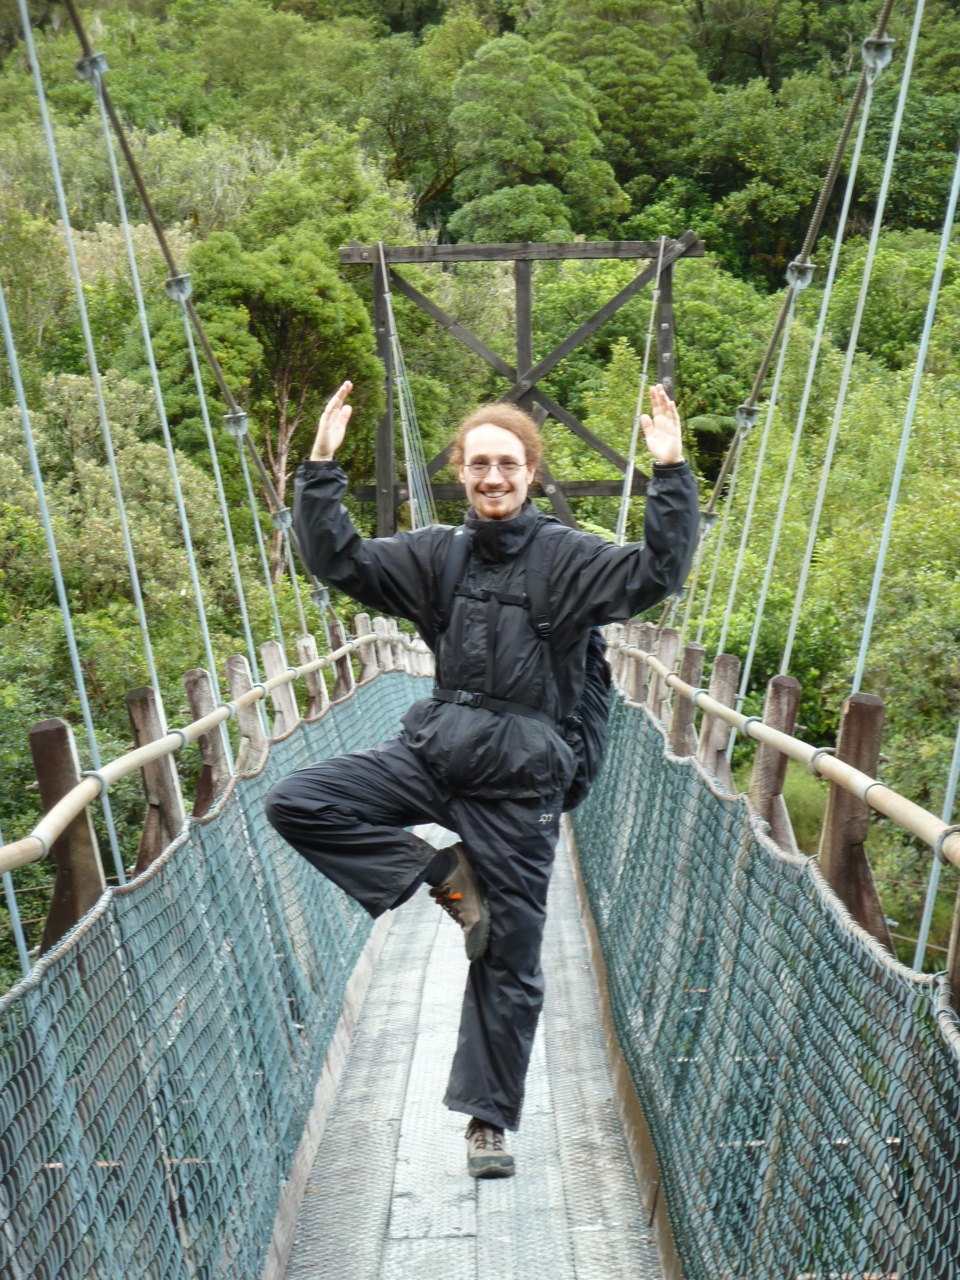
\includegraphics[height=.7\textheight,trim=0 100 0 200,clip]{img+txt/yoga_baum.jpg}
          \par\bigskip
          \begin{Huge}
            \Bmph{Vielen Dank.}
          \end{Huge}
        \end{center}
      }

      \note{
        \uzz{8:39 $\to$ nochmal zur Literatur, bis 8:40}{(10:05) Ende $\to$ nochmal zur Literatur}
        
        \par
      }
    \end{frame}
%%%  }

  % ------------------------------------------------------------------------------------------
    \begin{frame}
      \frametitle{Literatur für diesen Teil (Basis)}
      \begin{small}
        \begin{thebibliography}{99}
          \bibitem[Comon et al.\ 2008]{CDG+08}
%             Hubert Comon et al.\
            Hubert Comon, Max Dauchet, R\'emi Gilleron,
            Florent Jacquemard, Denis Lugiez, Christof L\"oding, Sophie Tison, Marc Tommasi.
            \newblock
            Tree Automata Techniques and Applications.
            \newblock
            \url{http://tata.gforge.inria.fr}\quad Nov.\ 2008.
            \newblock
            Kapitel 1\\
            Abschnitt 2.4 (Verbindung zu kontextfreien Wortsprachen)\\
%             Abschnitt 3.4.2 (Einschließung bei Termersetzungssystemen) \\
            Abschnitte 8.2.1, 8.2.2, 8.7 (Heckenaut.\ und XML-Schemasprachen)
          \bibitem[Bienvenu 2009]{Bie09}
            Meghyn Bienvenu.
            \newblock
            Automata on Infinite Words and Trees.
            \newblock
            Vorlesungsskript, Uni Bremen, WS 2009/10.
            \newblock
            \url{http://www.informatik.uni-bremen.de/tdki/lehre/ws09/automata/automata-notes.pdf}
            \newblock
            Kapitel 3
        \end{thebibliography}
        \par
      \end{small}

      \note{~}
    \end{frame}

  % ------------------------------------------------------------------------------------------
    \begin{frame}
      \frametitle{Literatur für diesen Teil (weiterführend)}
      \begin{small}
        \begin{thebibliography}{99}
          \bibitem[Br\"uggemann-Klein \& Wood 1998]{BW98}
            Anne Br{\"u}ggemann-Klein, Derick Wood.
            \newblock
            One-Unambiguous Regular Languages.
            \newblock
            Information and Computation, 142:1998, S.\ 182--206.
            \newblock
            \url{http://dx.doi.org/10.1006/inco.1997.2695}
            \newblock
            Grundlegende Resultate für deterministische reguläre Ausdrücke.          
        \end{thebibliography}
        \par
      \end{small}

      \note{~}
    \end{frame}

\mode<presentation>{
  {   
    \setbeamercolor{background canvas}{bg=black}
    \begin{frame}<handout:0>[plain]{}

      \note{~}
    \end{frame}
  }
}

\AtBeginSection{\frame{\frametitle{Und nun \dots}\tableofcontents[currentsection]}}
  

%     % ------------------------------------------------------------------------------------------
%     \begin{frame}
%       \frametitle{Ausblick}
% 
%       \dots
%       
%       \par\bigskip
%       \uncover<2>{%
%         \begin{center}
%           \begin{Huge}
%             \dblu{\textbf{Thank you.}}
%           \end{Huge}
%         \end{center}
%       }
%     \end{frame}

%   % ==============================================================================================
%   % ==============================================================================================
%   \appendix
%   
%     % ------------------------------------------------------------------------------------------
%     \begin{frame}
%       \frametitle{\dots}
%       \dots
%     \end{frame}

\end{document}
